%%%%%%%%%%%%%%%%%%%%%%%%%%%%%%%%%%%%%%%%%%%%%%%%%%%%%%%%%%%%%%%%%
% MUW Presentation
% LaTeX Template
% Version 1.0 (27/12/2016)
%
% License:
% CC BY-NC-SA 4.0 (http://creativecommons.org/licenses/by-nc-sa/3.0/)
%
% Created by:
% Nicolas Ballarini, CeMSIIS, Medical University of Vienna
% nicoballarini@gmail.com
% http://statistics.msi.meduniwien.ac.at/
%
% Customized for UAH by:
% David F. Barrero, Departamento de Automática, UAH
%%%%%%%%%%%%%%%%%%%%%%%%%%%%%%%%%%%%%%%%%%%%%%%%%%%%%%%%%%%%%%%%%

\documentclass[10pt,compress]{beamer} % Change 10pt to make fonts of a different size
\mode<presentation>

\usepackage[spanish]{babel}
\usepackage{fontspec}
\usepackage{tikz}
\usepackage{etoolbox}
\usepackage{xcolor}
\usepackage{xstring}
\usepackage{listings}

\usetheme{UAH}
\usecolortheme{UAH}
\setbeamertemplate{navigation symbols}{} 
\setbeamertemplate{caption}[numbered]

%%%%%%%%%%%%%%%%%%%%%%%%%%%%%%%%%%%%%%%%%%%%%%%%%%%%%%%%%%%%%%%%%
%% Presentation Info
\title[Introduction to Aritificial Intelligence]{Introduction to Artificial Intelligence}
\author{}
\institute{\asignatura}
\date{}
%%%%%%%%%%%%%%%%%%%%%%%%%%%%%%%%%%%%%%%%%%%%%%%%%%%%%%%%%%%%%%%%%


%%%%%%%%%%%%%%%%%%%%%%%%%%%%%%%%%%%%%%%%%%%%%%%%%%%%%%%%%%%%%%%%%
%% Descomentar para habilitar barra de navegación superior
\setNavigation
%%%%%%%%%%%%%%%%%%%%%%%%%%%%%%%%%%%%%%%%%%%%%%%%%%%%%%%%%%%%%%%%%

%%%%%%%%%%%%%%%%%%%%%%%%%%%%%%%%%%%%%%%%%%%%%%%%%%%%%%%%%%%%%%%%%
%% Configuración de logotipos en portada
%% Opacidad de los logotipos
\newcommand{\opacidad}{1}
%% Descomentar para habilitar logotipo en pié de página de portada
\renewcommand{\logoUno}{Images/isg.png}
%% Descomentar para habilitar logotipo en pié de página de portada
%\renewcommand{\logoDos}{Images/CCLogo.png}
%% Descomentar para habilitar logotipo en pié de página de portada
%\renewcommand{\logoTres}{Images/ALogo.png}
%% Descomentar para habilitar logotipo en pié de página de portada
%\renewcommand{\logoCuatro}{Images/ELogo.png}
%%%%%%%%%%%%%%%%%%%%%%%%%%%%%%%%%%%%%%%%%%%%%%%%%%%%%%%%%%%%%%%%%

%%%%%%%%%%%%%%%%%%%%%%%%%%%%%%%%%%%%%%%%%%%%%%%%%%%%%%%%%%%%%%%%%
%% FOOTLINE
%% Comment/Uncomment the following blocks to modify the footline
%% content in the body slides. 


%% Option A: Title and institute
\footlineA
%% Option B: Author and institute
%\footlineB
%% Option C: Title, Author and institute
%\footlineC
%%%%%%%%%%%%%%%%%%%%%%%%%%%%%%%%%%%%%%%%%%%%%%%%%%%%%%%%%%%%%%%%%

\begin{document}

%%%%%%%%%%%%%%%%%%%%%%%%%%%%%%%%%%%%%%%%%%%%%%%%%%%%%%%%%%%%%%%%%
% Use this block for a blue title slide with modified footline
{\titlepageBlue
    \begin{frame}
        \titlepage
    \end{frame}
}

\begin{frame}[plain]{}
	\begin{block}{Objectives}
		\begin{enumerate}
		\item Think over the meaning of intelligence
		\item Understand Artificial Intelligence (AI) as a Computer Science discipline
		\item Describe the historical roots of AI
		\item Elemental AI terminology
		\item Introduce some AI applications
		\IfStrEq{\modo}{MASTER-ESPACIO}{
			\item Applications of AI in space
		}{}
		\end{enumerate}
	\end{block}

	\begin{block}{Objectives}
	Russell, S., Norvig, P. (1995). \textit{Artificial Intelligence: A modern approach}. Prentice-Hall.
	\end{block}
\end{frame}

{ \disableNavigation{white}
\begin{frame}[shrink]{Table of Contents}
 \frametitle{Table of Contents}
 \tableofcontents
  % You might wish to add the option [pausesections]
\end{frame}
}

\begin{frame}[plain]{}
	\begin{columns}
 	   \column{.50\textwidth}
		\begin{block}{}
			\centering What is intelligence?
		\end{block}
	\end{columns}
\end{frame}

\begin{frame}[plain]{}
	\begin{tabular}{ll}
		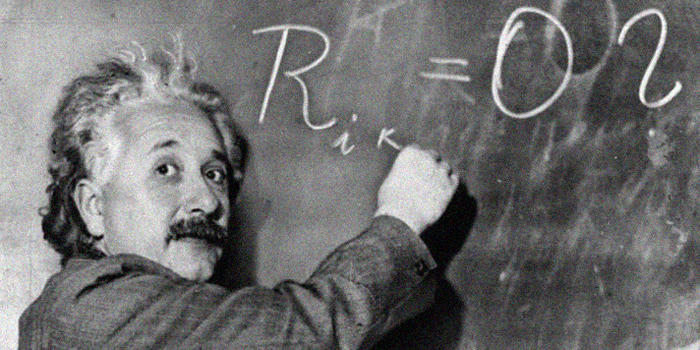
\includegraphics[width=0.4\linewidth]{figs/einstein.jpg} & 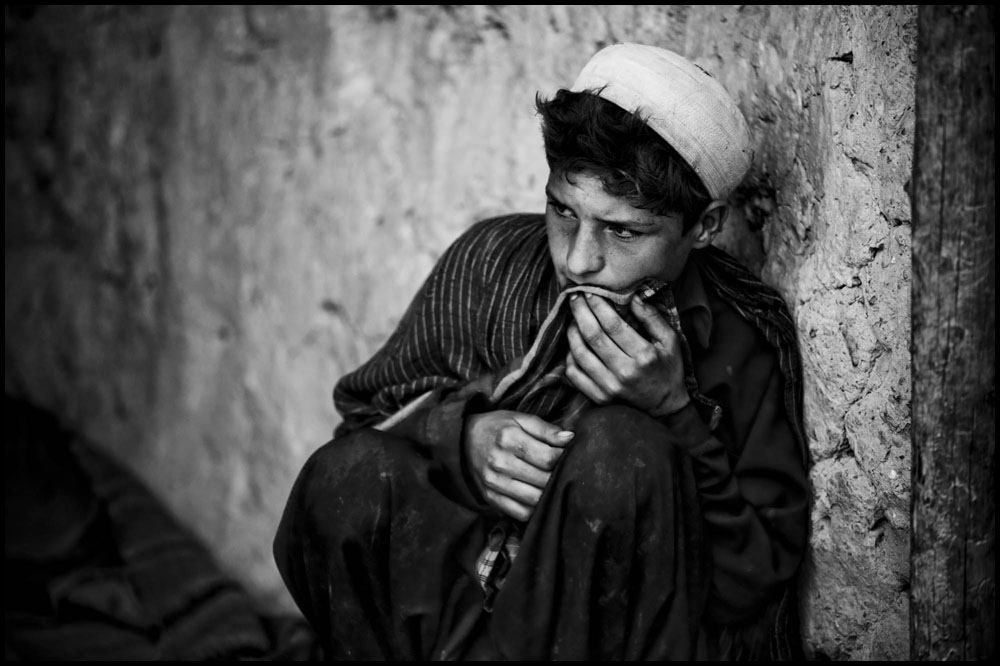
\includegraphics[width=0.4\linewidth]{figs/empatia.jpg} \\ 
  	 & \tiny{\href{https://www.flickr.com/photos/zoriah/5741923543/in/photolist-9KoRPM-4uuLxz-jysFM-7MFnqH-azjwr-GcuDW-a13kEq-7jSbrA-4mNb6B-4FSbEW-8vEXcj-8P76u6-5gzcMn-uRkEwG-8sY6E2-iXsoin-52Ziee-8nZs5P-nPNSsY-4pnbRo-cqAWZS-4xLGVS-4VabYG-iYCeww-dRSst2-4pC3KR-EWEMN-eoZgzx-d7q5Vj-5CV6Zm-d7qgE9-4Z444F-4K9Ycz-6Em2P-fKWK3J-38tp9W-8P4JXn-7j3p1L-5z8FrL-srdMQB-orscLa-7rrrPy-dRKSp3-AmNGy6-6iobyU-8S4w4d-kiZssW-dAEM7S-5gDxL9-dDNBfB/}{(Source)}}     \\ 
		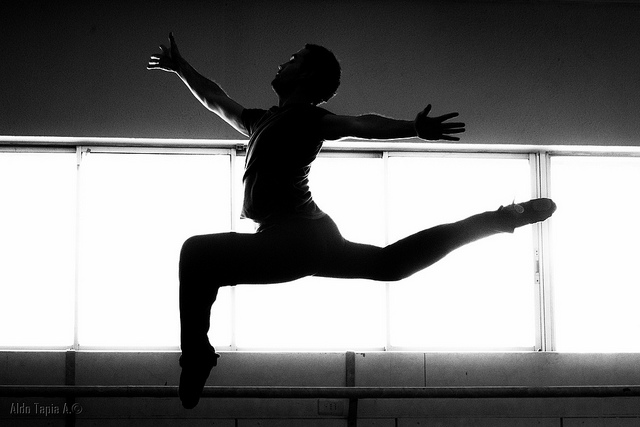
\includegraphics[width=0.4\linewidth]{figs/jump.jpg} & 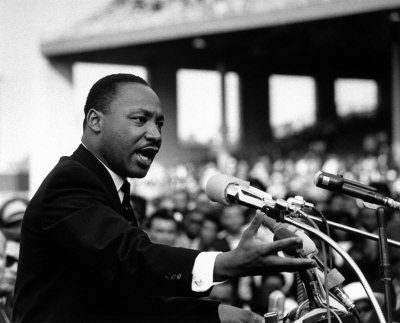
\includegraphics[width=0.4\linewidth]{figs/martin-luther-king.jpg} \\ 
  	\tiny{\href{https://www.flickr.com/photos/aldotapia/8171337460/in/photolist-ds5eWC-8NG6LL-cH4tWE-cH4txy-cH4ts5-8NG7aU-cH4sZE-cuYmRf-8ND1J6-8ND1GH-cbt1vd-9pQm6z-cbt2xS-cbsYuJ-cbsYFd-cbsXkb-cbt1LW-nwrd7b-CQGFK-6ACqW6-rfj43P-chqF2s-5ggjXu-8ND1V2-8NG77f-6B7mzx-8NG7eo-8NG75L-8ND1Mr-8ND1Q6-5345tB-zDkboz-ceqAoY-jhv4Zb-BixwUf-9KVNqY-8vxrrD-sTXGfX-fkuc7V-8vxrqM-CQGFW-ceqDd5-aUoPiZ-ceqGTG-5g3N1u-cdJqjq-e58ZyN-3remmb-95eTYM-ezDHvV/}{(Source)}} &   \\ 
	\end{tabular}
\end{frame}

\begin{frame}[plain]{}
	\vspace{-0.4cm}
	\begin{center}
	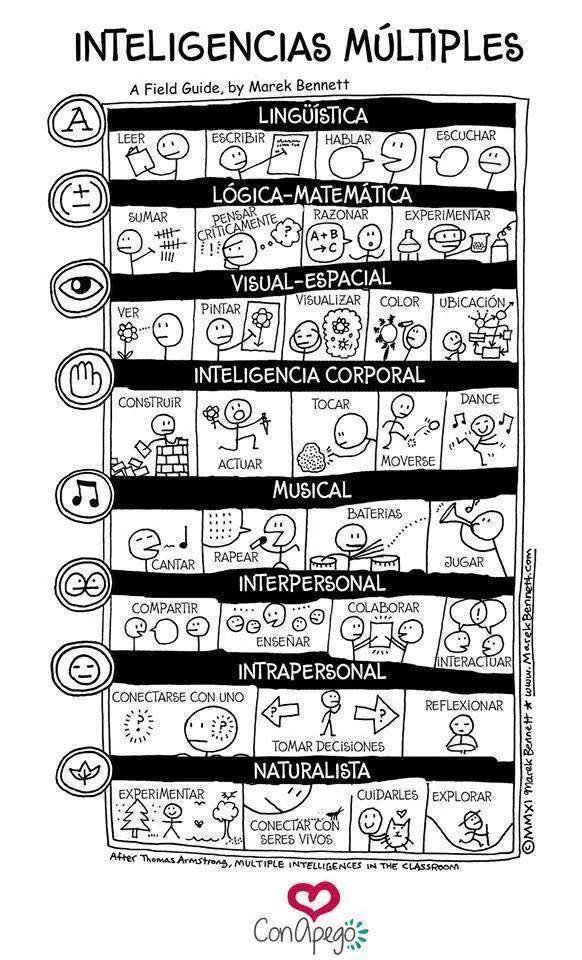
\includegraphics[width=0.6\linewidth]{figs/inteligencia.jpg}
	\end{center}
\end{frame}

\section{Introduction}

\subsection{Intelligence}
\begin{frame}{Introduction}{Intelligence (I)}
	\begin{columns}
 	   \column{.80\textwidth}
		\begin{block}{Definition of intelligence}
			``\textit{A very general mental capability that, among other things, includes the ability to reason, pose, solve problems, think abstractly, understand complex ideas, learn quickly and learn from experience}''\\
			\begin{flushright}Gottfredson, 1997\end{flushright}
		\end{block}
	\end{columns}
	\bigskip
	Not only from books, limited academic ability, or make good tests
	\begin{itemize}
		\item It reflects a broader and deeper capacity
	\end{itemize}
\end{frame}

\begin{frame}{Introduction}{Intelligence (II)}
	Alternative definition: Capacity to \textbf{learn} and \textbf{solve} problems (Websters dictionary)
	\begin{itemize}
		\item The ability to solve novel problems
		%\item The ability to act \textbf{rationally}
		%\item The ability to act \textbf{like humans}
	\end{itemize}
\end{frame}

\subsection{Artificial Intelligence}
\begin{frame}{Introduction}{Artificial Intelligence (I)}
	\begin{columns}
 	   \column{.80\textwidth}
		\begin{block}{Definition of AI}
			Build machines that perform tasks that were previously performed by human beings
		\end{block}
	\end{columns}
	\bigskip
	\begin{itemize}
		\item People process information slowly but in parallel
		\item Computers are incredibly fast but essentially linear
		\item It reflects a broader and deeper capacity
		\item Intelligence requires knowledge: \alert{Learning}
	\end{itemize}
\end{frame}

\begin{frame}{Introduction}{Artificial Intelligence (II)}
	Alternative definition: \textbf{Understand} and \textbf{build} intelligent entities
	\begin{itemize}
		\item Understand: Use computers to study intelligence (\textit{Science})
		\item Build: Solve real problems using knowledge and reasoning (\textit{Engineering})
		\item Intelligent entity = \alert{agent}
	\end{itemize}
	AI deals with \textbf{algorithms} and \textbf{knowledge representation}
	\begin{itemize}
		\item AI is not restricted to any programming language
	\end{itemize}
\end{frame}

\subsection{Approaches to Artificial Intelligence}
\begin{frame}{Introduction}{Approaches to Artificial Intelligence (I)}
	Two goals: Humanity and rationality
	\begin{itemize}
		\item Human: Like human beings
		\item Rational: Doing the right thing
		\item The right thing: What is expected to maximize goal achievement, given the available information
	\end{itemize}
	Two dimensions: Processes (thinking) and result (acting)

	\vspace{-0.5cm}
	\begin{center}
	\begin{tabular}{|p{5cm}|p{5cm}|}\hline
	\textbf{Thinking humanly} 	& \textbf{Thinking rationally} \\\hline
	Theories about internal activities of the brain $\Rightarrow$ Neuscience & What are correct arguments? $\Rightarrow$ Logics\\\hline
	\textbf{Acting humanly} & \textbf{Acting rationally} \\\hline
	Can machines think? & Rational agents \\\hline
	\end{tabular}
	\end{center}
\end{frame}

\begin{frame}{Introduction}{Approaches to Artificial Intelligence (II)}
	\begin{columns}
 	   \column{.50\textwidth}
	   \begin{center}
	   	\textbf{Thinking humanly}
	   \end{center}
	   \begin{itemize}
	   \item Scientific theory of internal activities of the brain
	   \item How to validate?
	   		\begin{itemize}
	   		\item Predicting behavior of humans (\textbf{Cognitive science})
	   		\item Identification of neurological data (\textbf{Neuroscience})
	   		\end{itemize}
	   \end{itemize}
	   
 	   \column{.50\textwidth}
	   	\begin{center}
	   		\textbf{Acting humanly}
	   	\end{center}
	   	Can machines think? Test needed: \alert{Turing test}\\
		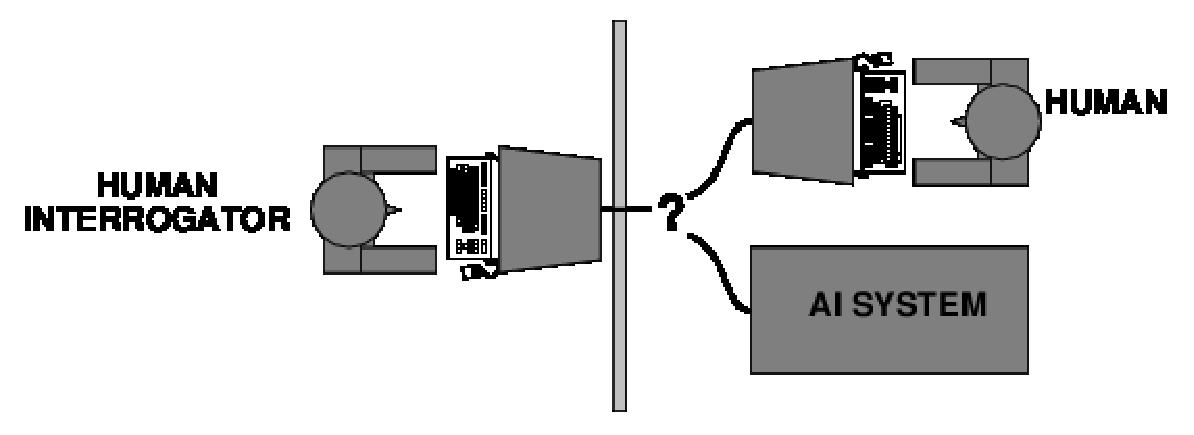
\includegraphics[width=\linewidth]{figs/turing.eps}\\
		Proposed by Alan Turing (yes, that Turing!)
	\end{columns}
\end{frame}

\begin{frame}[fragile]{Introduction}{Approaches to Artificial Intelligence (III)}
	Real Turing test at the Royal Society (2014)
	\tiny{
	   	\begin{exampleblock}{Chat 1} % DFBARRERO: Humano
		\begin{verbatim}
[16:28:55] Judge: how tall are you
[16:29:18] Entity: almost 6 feet tall
[16:29:46] Judge: how heavy are you
[16:30:12] Entity: just over ten stone
[16:30:47] Judge: what is your gender
[16:30:59] Entity: male
[16:31:45] Judge: what is your bmi
[16:31:54] Entity: i have no clue
		\end{verbatim}
		\end{exampleblock}
	   	\begin{exampleblock}{Chat 2} % DFBARRERO: Este es el bot, Eurine Goosman
		\begin{verbatim}
[16:29:04] Judge: how tall are you
[16:29:10] Entity: My height is about 160 cm – it’s 5 feet 4 inches.
[16:29:37] Judge: how heavy are you
[16:29:59] Entity: My grandfather taught me not to disclose non-solicited information about
myself. Like on the question ‘Do you have watch’ – never tell time, but answer ‘Yes’ or
‘No’. I always follow his advice. And I forgot to ask you where you are from ...
[16:31:09] Judge: what is your gender
[16:31:17] Entity: I’m a young boy, if you care to know. And not very ugly, by the way!
		\end{verbatim}
		\end{exampleblock}
	}
	\href{(Source)}{http://www.tandfonline.com/doi/pdf/10.1080/0952813X.2015.1055826}
\end{frame}


\begin{frame}[plain]{Introduction}{Approaches to Artificial Intelligence (IV)}
	\vspace{-0.5cm}
	\begin{columns}
 	   \column{.50\textwidth}
		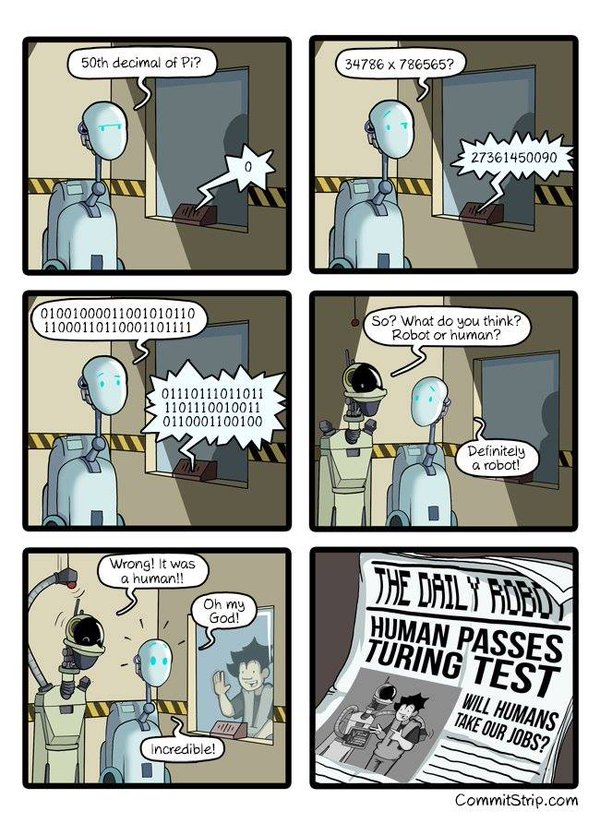
\includegraphics[width=\linewidth]{figs/turingRobot.jpg}
	\end{columns}
\end{frame}

\begin{frame}{Introduction}{Approaches to Artificial Intelligence (IV)}
	\begin{columns}
 	   \column{.50\textwidth}
	   \begin{center}
	   		\textbf{Thinking rationally}
	   \end{center}

	   \begin{itemize}
	   \item ``Laws of thought''
	   \item Aristotle: What are correct arguments? $\Rightarrow$ \textbf{Logic}
	   \item Connects Philosophy, Mathematics and AI
	   \item Problems
	   		\begin{itemize}
	   		\item Not all intelligent behavior is deliberative
	   		\item What is the purpose of thinking?
	   		\end{itemize}
	   \end{itemize}
	   
 	   \column{.50\textwidth}
	   	\begin{center}
	   		\textbf{Acting rationally}
	   	\end{center}
	   	\textbf{Agent}: Entity that perceives and acts
		\begin{itemize}
			\item A robot may be seen as an phisical agent
			\item Amazon recommender system
			\item Spam filter
		\end{itemize}
		Computational constrains: Design the best program with available resources
	\end{columns}
\end{frame}

\subsection{Related fields}
\begin{frame}{Introduction}{Related fields}
	\vspace{-0.8cm}
	\begin{center}
	\begin{tabular}{|p{2.5cm}|p{8cm}|}\hline
	Philosophy  & Logic, methods of reasoning, mind as physical system, foundations of learning, language, rationality\\\hline
	Mathematics & Formal representation, proof algorithms, computation, (un)decidability, (in)tractability, probability\\\hline
	Probability & Modeling uncertainty, learning from data\\\hline
	Economics   & Utility, decision theory, rational economic agents\\\hline
	Neuroscience& Neurons as information processing units\\\hline
	Psychology  & How do people behave, process cognitive information, represent knowledge\\\hline
	Computer Engineering & Build fast computers\\\hline
	Control theory & Optimization\\\hline
	Linguistics & Knowledge representation, grammars\\
	 \hline
	\end{tabular}
	\end{center}
\end{frame}

%\begin{frame}{Introduction}{Related fields: Philosophy (I)}
%	Questions
%	\begin{itemize}
%		\item Are there formal rules to draw valid conclusions? 
%		\item Where does knowledge come from? 
%		\item How to go from knowledge to action?
%	\end{itemize}
%	Philosophical schools
%	\begin{itemize}
%		\item Syllogisms: Aristotle. Drawing mechanically  conclusions from initial premises
%		\item Dualism: Descartes. A part of the mind that is outside of nature%. %Animals do not possess this dual quality and nor machines 
%		\item Materialism: The brain operations performed in accordance Physics 
%		\item ...
%	\end{itemize}
%\end{frame}

%\begin{frame}{Introduction}{Related fields: Philosophy (II)}
%	Philosophical schools (cont.)
%	\begin{itemize}
%		\item ...
%		\item Empirical: Nothing exists in the mind that has not passed through the senses 
%		\item Induction: The general rules are obtained by exposure to repeated associations between their elements 
%		\item Logical Positivism: All knowledge can be characterized by related logical theories
%		\item Confirmation theory: Try to explain how knowledge is obtained from experience
%	\end{itemize}
%\end{frame}

%\begin{frame}{Introduction}{Related fields: Mathematics (I)}
%	Questions
%	\begin{itemize}
% 		\item What formal rules to follow to obtain valid conclusions? 
%		\item What can be computed? 
%		\item How to reason with uncertainty?
%	\end{itemize}
%	Disciplines
%	\begin{itemize}
%		\item Formal Logic: Mathematical development through propositional logic or Boolean 
%		\item Algorithm: The first was the trivial Euclidean algorithm for calculating the MCD. Algorithms for logical deductions 
%		\item Incompleteness theorem: There are true statements that cannot be decidable (can not be validated by algorithms) 
%		\item ...
%	\end{itemize}
%\end{frame}

%\begin{frame}{Introduction}{Related fields: Mathematics (II)}
%	Disciplines (cont.)
%	\begin{itemize}
%		\item ...
%		\item Intractability: Problems in the time needed to resolve individual cases grow exponentially with the size of the cases 
%		\item NP-Completeness: A method for identifying intractable problems 
%		\item Probability: Support the processing of uncertainty measurements	
%	\end{itemize}
%\end{frame}


%\begin{frame}{Introduction}{Related fields: Economy}
%	How to make decisions to maximize efficiency?
%	\begin{itemize}
%		\item Decision Theory: Combines probability theory with utility theory 
%		\item Game Theory: In some games, a rational agent should act randomly, or at least, apparently random
%		\item Operations Research: Optimization and complex decisions making 
%		\item Satisfaction: Making decisions that are ``good enough''
%	\end{itemize}
%\end{frame}

%\begin{frame}{Introduction}{Related fields: Neuroscience}
%How the brain processes information?
%	\begin{itemize}
%		\item Neuroscience: Study the neurological system and especially the brain. The exact way in which the brain generates thoughts 
%		\item Neurons: The brain consists of nerve cells called neurons that have been observed and studied individually
%	\end{itemize}
%\end{frame}

%\begin{frame}{Introduction}{Related fields: Psycology}
%How humans and animals think and act?
%	\begin{itemize}
%	\item Behaviorism: Rejects any theory in which mental processes are involved. They insisted on the exclusive study of objective measures of perceptions (stimuli) and the resulting actions (responses) 
%	\item Cognitive Psychology: Conceptualization of the brain as an information processing device. It emphasizes that perception involves some kind of logical inference unconscious 
%	\item Cognitive Science: Using computer models to model the psychology of memory, language and logical thinking
%	\end{itemize}
%\end{frame}

%\begin{frame}{Introduction}{Related fields: Computer Engineering}
%How can you build an efficient computer?
%	\begin{itemize}
%	\item AI besides intelligence also needs a machine (computer) 
%	\item Hardware: Oncreasing processing speed and storage capacity 
%	\item Software: Operating systems, programming languages and modern tools to write programs%. AI research has generated many important ideas: timeshare, interpreters, graphical interfaces, rapid development environments, symbolic, functional, dynamic, object-oriented programming.
%	\end{itemize}
%\end{frame}

%\begin{frame}{Introduction}{Related fields: Cybernetics and Control Theory}
%How can artifacts operate under their own control?
%	\begin{itemize}
%	\item Control theory: See the emergent deterministic behavior as a regulatory mechanism that attempts to minimize the ```error''% (the difference between the current state and the goal) 
%	\item Cybernetics: Mathematical and computational cognitive models 
%	\item Objective Function: Contemporary Theory based control design systems that maximize an objective function over time
%	\end{itemize}
%\end{frame}

%\begin{frame}{Introduction}{Related fields: Linguistics}
%     How language relates to Linguistics
%	\begin{itemize}
%	\item Computational Linguistics: Convergence between modern linguistics and AI (Natural Language Processing)
%	\end{itemize}
%\end{frame}

\section{History}
\subsection{Timeline}
\begin{frame}{History}{Timeline (I)}
	\begin{description}
	\item[1943] Early beginnings
		\begin{itemize}
		\item McCulloch \& Pitts Boolean circuit model of brain
		\end{itemize}
	\item[1950] Turing 
		\begin{itemize}
		\item Turing's ``Computing Machinery and Intelligence''
		\end{itemize}
	\item[1952] Look, Ma, no hands!
	\item[1956] Birth of AI
		\begin{itemize}
		\item Dartmouth meeting: ``Artificial Intelligence'' adopted
		\end{itemize}
	\end{description}
\end{frame}

\begin{frame}{History}{Timeline (II)}
	\begin{description}
	\item[1950s] Early AI programs
		\begin{itemize}
		\item Samuel's checkers program
		\item Newell \& Simon's Logic Theorist
		\end{itemize}
	\item[1955-65] Great enthusiasm
		\begin{itemize}
		\item Newell and Simon: GPS, general problem solver
		\item McCarthy: Invention of LISP
		\end{itemize}
	\item[1966-73] Reality dawns
		\begin{itemize}
		\item AI discovers computational complexity
		\item Limitations of existing neural networks methods identified
		\item Neural network research almost disappears
		\end{itemize}
	\end{description}
\end{frame}

\begin{frame}[plain]{History}{Timeline (III)}
	\begin{description}
	\item[1969-79] Adding domain knowledge
		\begin{itemize}
		\item Early development of knowledge-based systems
		\end{itemize}
	\item[1986-] Raise of Machine Learning
		\begin{itemize}
		\item Neural Networks return to popularity
		\item Major advances in Machine Learning and its applications
		\end{itemize}
	\item[1990-] Role of uncertainty
		\begin{itemize}
		\item Bayesian networks for knowledge representation
		\end{itemize}
	\item[1995-] AI becomes a science
		\begin{itemize}
		\item Integration of learning, reasoning and knowledge representation
		\item AI used in vision, language, data mining, etc
		\end{itemize}
	\item[2000-] Popularity of Soft Computing / Bioinspired algorithms
	\item[2010-] Machine Learning meets large databases: Big Data
	\end{description}
\end{frame}

\begin{frame}{History}{Timeline (IV)}
	\begin{center}
		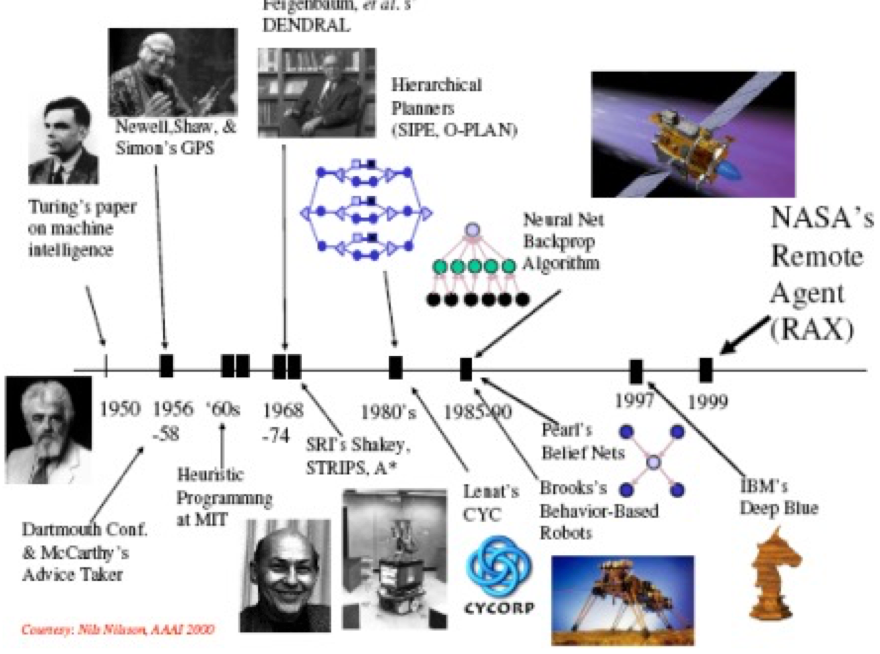
\includegraphics[width=0.8\linewidth]{figs/history.png}
	\end{center}
\end{frame}

\subsection{Success milestones}
\begin{frame}{History}{Success milestones}
	\begin{itemize}
	\item Deep Blue defeated Garry Kasparov in 1997 
	\item Proved the Robbins conjecture, unsolved for decades 
	\item No hands across America 
	\item During the 1991 Gulf War, US forces deployed an AI logistics planning and scheduling program that involved up to 50,000 vehicles, cargo, and people 
	\item NASA's on-board autonomous planning program controlled the scheduling of operations for a spacecraft 
	\item Proverb solves crossword puzzles better than most humans
	\item Robot driving: DARPA grand challenge 2003-2007
	\item 2006: Face recognition software available in consumer cameras
	\item 2011: IBM Watson defeats human players in Jeopardy!
	\item 2016: First AI to defeat a Go human champion
	\end{itemize}
\end{frame}

\section{AI applications}
\subsection{2001: A Space Odyssey}

\begin{frame}{AI applications}{2001: A Space Odyssey (I)}
	\begin{columns}
 	   \column{.70\textwidth}
			2001: Space Odyssey
			\begin{itemize}
			\item Claimed as the best (and most realistic) sci-fi movie ever
			\item Filmed in 1969 by Stanley Kubrick
			\item Relates a journey to Jupiter (among many other things)
			\end{itemize}
			\href{https://www.youtube.com/watch?v=XHjIqQBsPjk}{(Video trailer)}
 	   \column{.30\textwidth}
		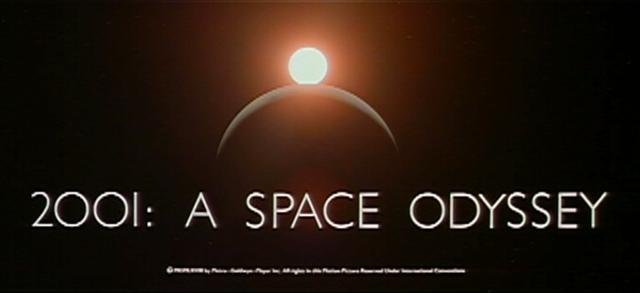
\includegraphics[width=\linewidth]{figs/kubrick1.jpg}\\
		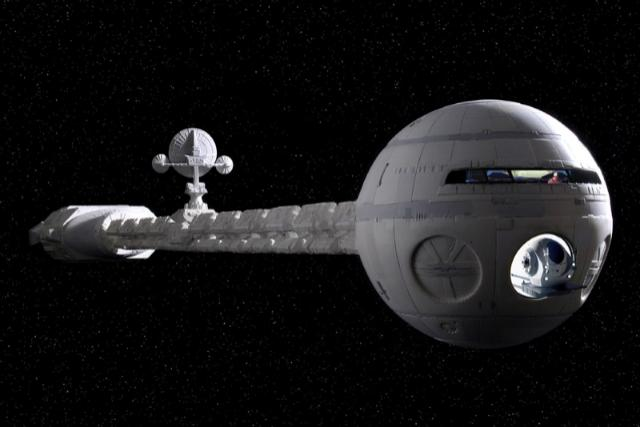
\includegraphics[width=\linewidth]{figs/2001-nave.jpg}
	\end{columns}
\end{frame}

\begin{frame}{AI applications}{2001: A Space Odyssey (II)}
	\begin{columns}
 	   \column{.05\textwidth}
 	   \column{.65\textwidth}
			The main character is HAL 9000
			\begin{itemize}
			\item HAL is an AI that controls an intelligent spaceship (an agent)
			\end{itemize}
			HAL has very advanced features
			\begin{itemize}
			\item Play chess
			\item Speak easily with the crew
			\item Understand the emotions of the crew
			\item Display emotions
			\item Navigate the ship
			\item Diagnose on-board problems
			\item Make life-and-death decisions
			\item Recognize the crew faces
			\end{itemize}
 	   \column{.3\textwidth}
	   	\begin{center}
		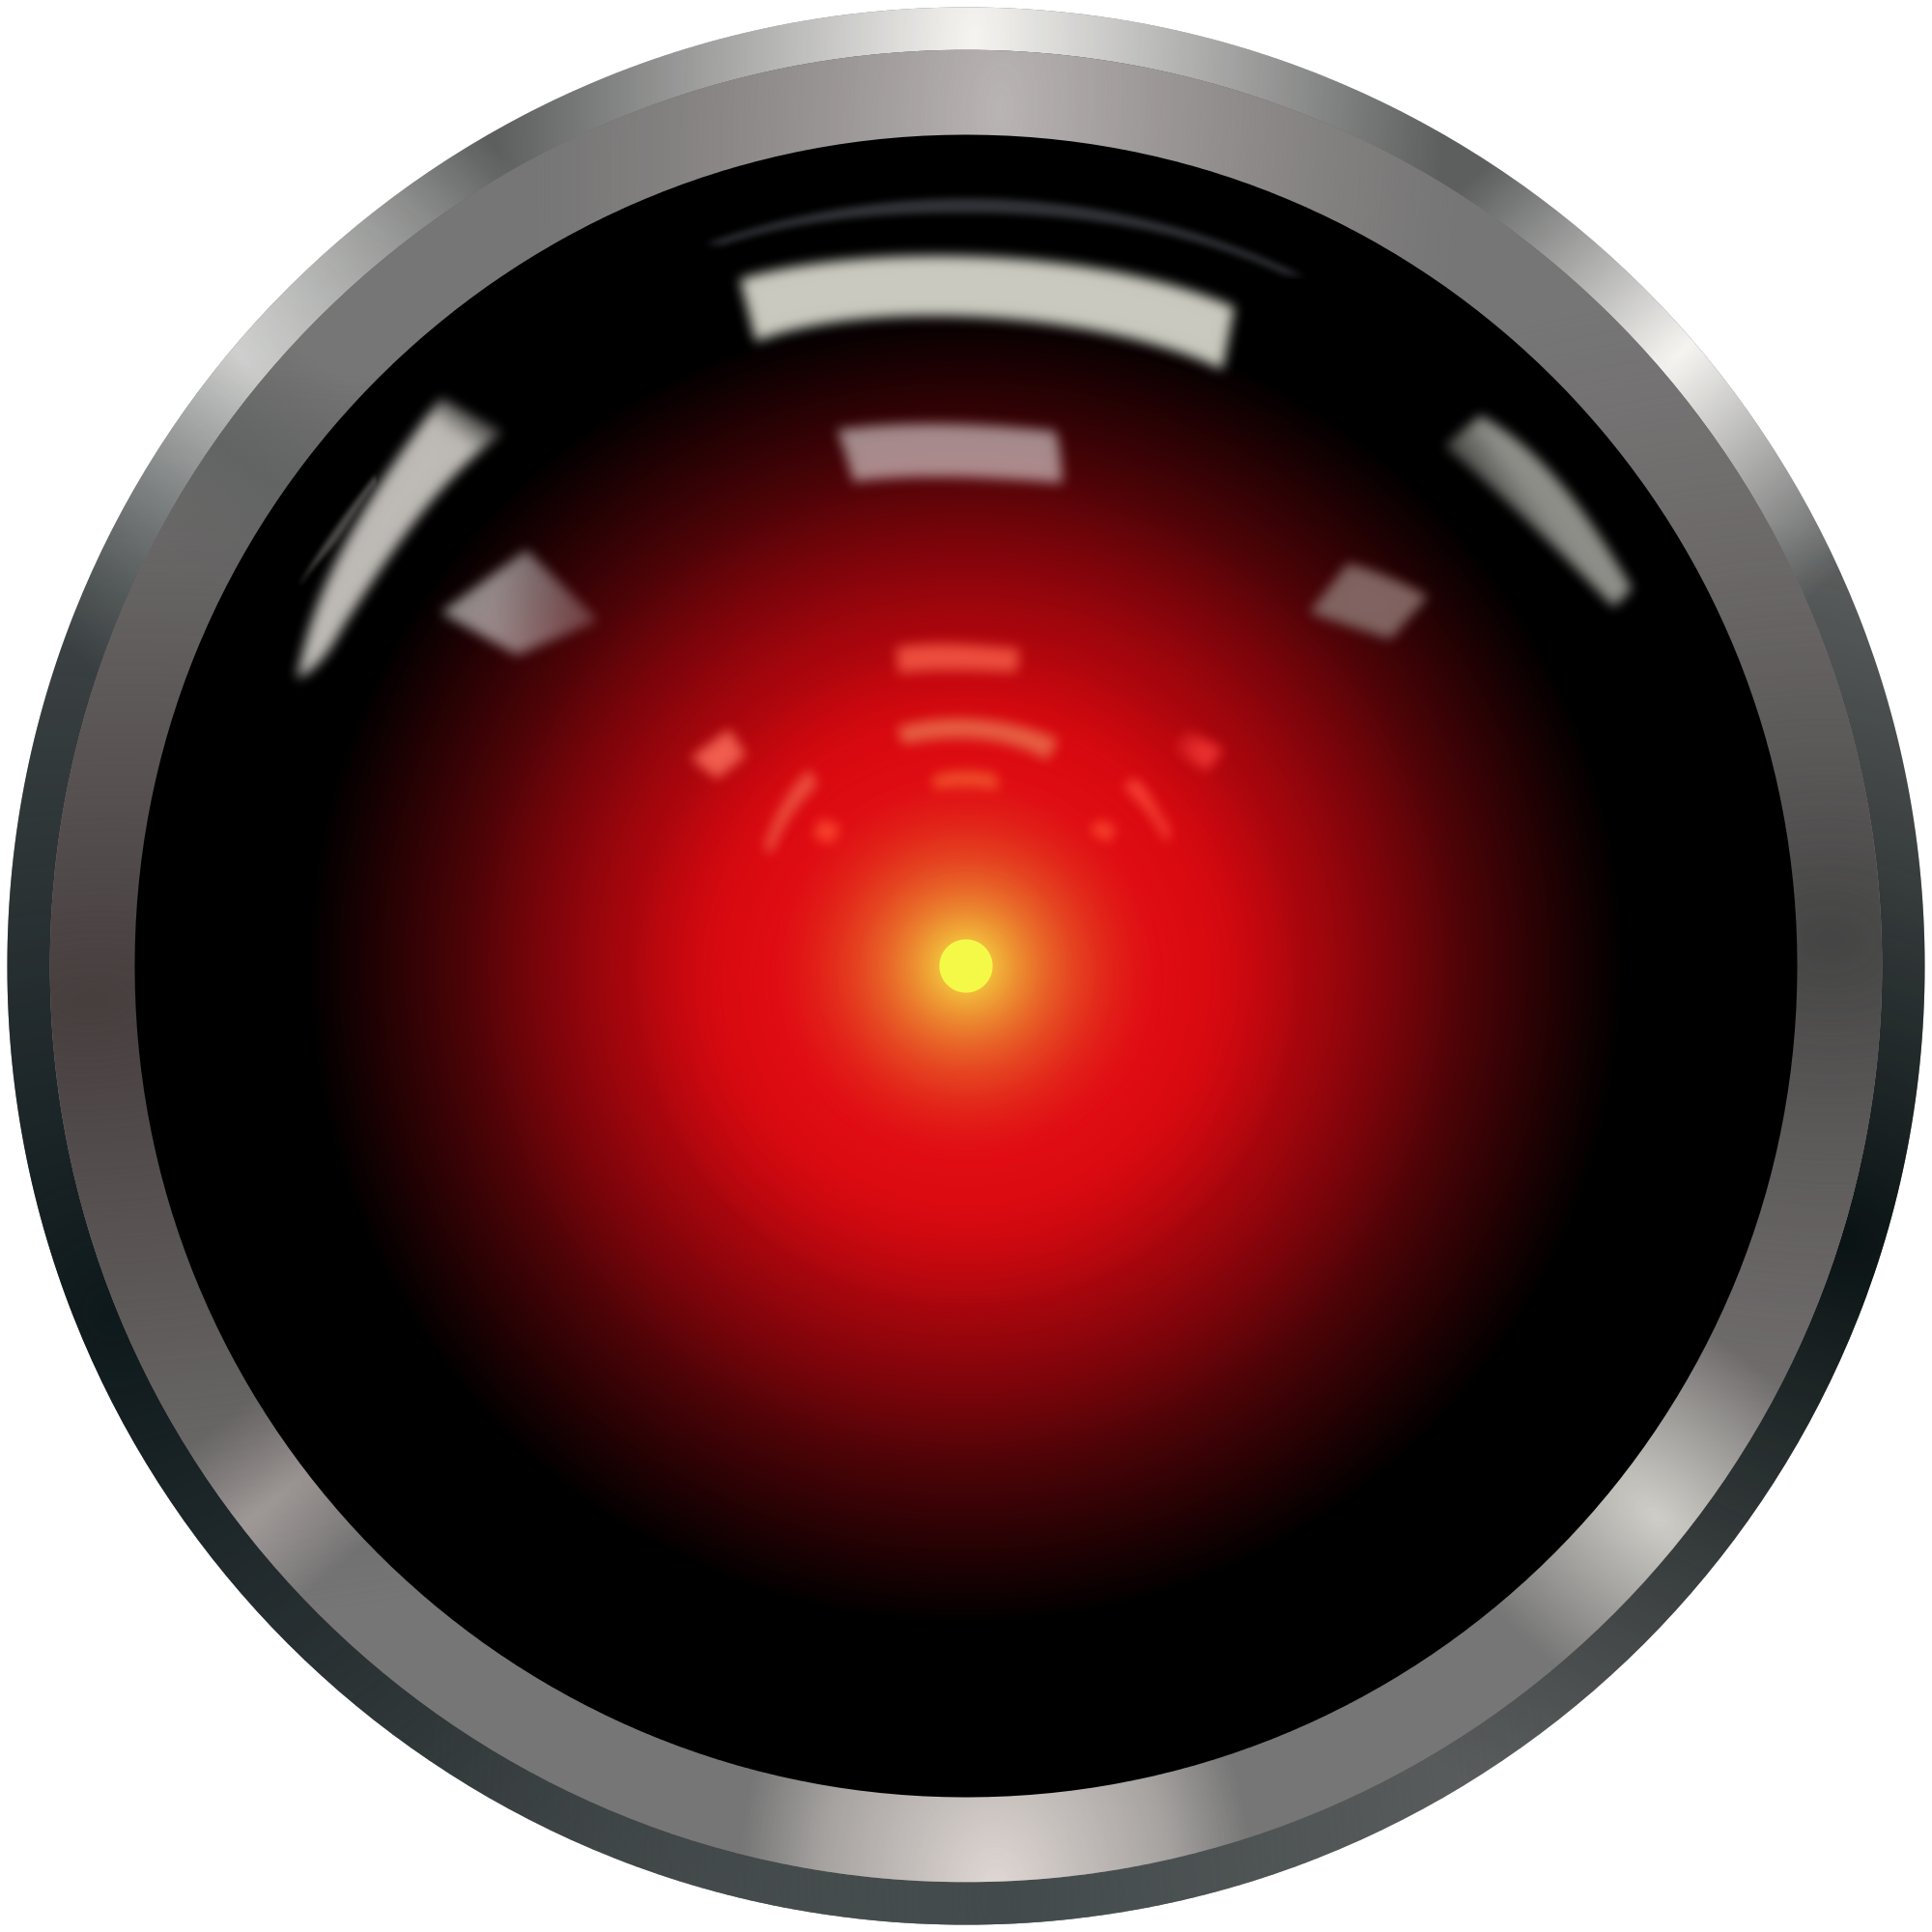
\includegraphics[width=0.8\linewidth]{figs/hal.png}
		\end{center}
		\begin{block}{}
			HAL was sci-fi in 1969 ... Is it still sci-fi?
		\end{block}
 	   \column{.05\textwidth}
	\end{columns}
\end{frame}

\subsection{Building HAL}
\begin{frame}{AI applications}{Building HAL}
	Imagine we want to build HAL ... What would we need?
	\begin{itemize}
		\item Fast hardware?
		\item Chess-playing at grandmaster level?
		\item Speech interaction?
		\item Learning?
		\item Image recognition and understanding?
		\item Planning and decision-making?
	\end{itemize}
	Let's analyze them
\end{frame}

\begin{frame}{AI applications}{Building HAL: Hardware (I)}
	How complicated is our brain?
	\begin{itemize}
		\item A neuron is the basic information processing unit
		\item Arround $10^{12}$ neurons in a human brain with ($10^{14}$) synapses 
		\item Processing time: $1 ms$
	\end{itemize}
	How complex can we make computers?
	\begin{itemize}
		\item $10^8$ or more transistors per CPU
		\item Supercomputers with thousands of CPUs
		\item Processing time: $10^{-9}s$
	\end{itemize}
\end{frame}

\begin{frame}{AI applications}{Building HAL: Hardware (II)}
	\begin{columns}
 	   \column{.60\textwidth}
	\begin{center}
		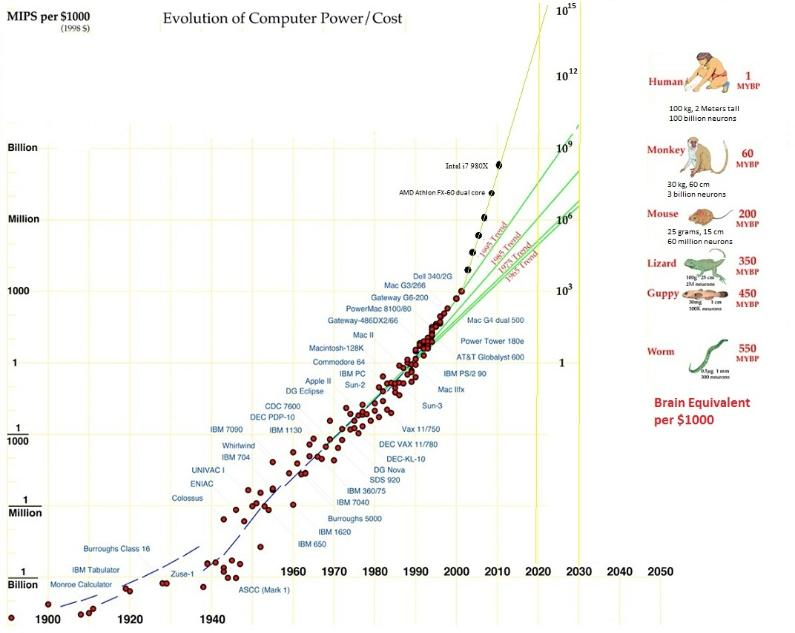
\includegraphics[width=\linewidth]{figs/power.jpg}\\
		\tiny{\href{http://www.sjef.nu/a-basic-introduction-to-singularity-skepticism/}{(Source)}}
	\end{center}
 	   \column{.40\textwidth}
	Conclusion
	\begin{itemize}
		\item YES, in a future we will have computers with as many processing units than human brains
		\begin{itemize}
		\item But, with fewer interconnections, and much faster
		\end{itemize}
		\item Processing power does not make behave like a brain
	\end{itemize}
	\end{columns}
\end{frame}

\begin{frame}{AI applications}{Building HAL: Chess (I)}
	Chess is a classic benchmark in AI
	\begin{itemize}
		\item AI techniques: Classic search
	\end{itemize}

	\vspace{-0.4cm}

	\begin{center}
		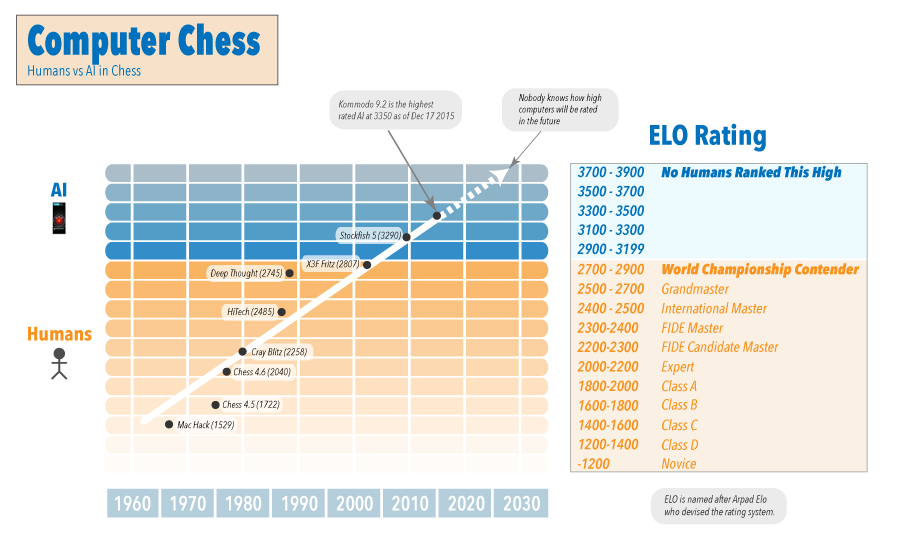
\includegraphics[width=0.7\linewidth]{figs/elo.png}\\
		\tiny{\href{http://www.statisticsviews.com/details/feature/8791241/Artificial-Intelligence-Solving-the-Chinese-Room-Argument.html}{(Source)}}
	\end{center}

	\vspace{-0.6cm}

	Conclusion: YES
\end{frame}

\begin{frame}{AI applications}{Building HAL: Chess (II)}
	\vspace{-2cm}

	\begin{center}
		
\includegraphics[width=0.4\linewidth]{figs/alphago.png}
	\end{center}

	\vspace{-0.2cm}
	In 2015, an AI beats the best human Go player
	\begin{itemize}
		\item Historic mildstone
	\end{itemize}
	Go is much harder from AI perspective
	\begin{itemize}
		\item Huge branching factor
		\item Fuzzy heuristics
	\end{itemize}
	AI techniques
	\begin{itemize}
		\item Monte-Carlo Search Trees
		\item Deep neural networks
	\end{itemize}
	Next challenge: StarCraft II

	\vspace{-4cm}
	\begin{columns}
 	   \column{.70\textwidth}
 	   \column{.30\textwidth}
		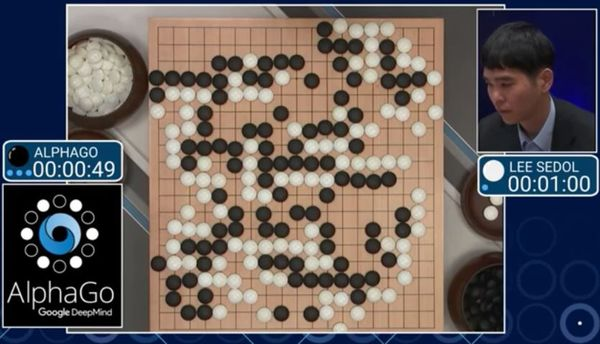
\includegraphics[width=\linewidth]{figs/leesedol.jpg}
	\end{columns}
\end{frame}

\begin{frame}{AI applications}{Building HAL: Speech synthesis}
	Three different problems to make computers talk
	\begin{itemize}
		\item Speech synthesis, speech recognition and speech understanding
	\end{itemize}
	Speech synthesis: Generate sound from text
	\begin{itemize}
		\item Translate text to phonemas: “fictitious”  $\Rightarrow$ fik-tish-es
		\item Generate sound from phonema: "tish" $\Rightarrow$ Sound
	\end{itemize}
	Difficulties
	\begin{itemize}
		\item This approach makes sounds unnatural
		\item Sounds are not indepentent (almost solved)
		\item Show emotions, emphasis, semantic-aware pronuntiation
	\end{itemize}
	Conclusion
	\begin{itemize}
		\item YES for words
		\item NO for complete sentences
	\end{itemize}
\end{frame}

\begin{frame}{AI applications}{Building HAL: Speech recognition}
\footnotesize{
	Speech recognition: Map sounds into a list of words
	\begin{itemize}
		\item Classic (and difficult) problem in AI
		\item Techniques: Neural networks, Hidden-Markov Chains, Deep Learning, ...
	\end{itemize}
	Recognizing single words from a small vocabulary
	\begin{itemize}
		\item Numbers, city numbers, names, ...
		\item Highly successfull solutions ($99\%$ accuracy)
	\end{itemize}
	Recognizing normal speech is much more difficult
	\begin{itemize}
		\item Large vocabularies
		\item Continous sound (detect word boundaries)
		\item Humans use context to recognize speech
		\item Background noise, accents, other speakers, ...
		\item Modern systems with $60\%$-$70\%$ accuracy
	\end{itemize}
	Conclusion: YES for restricted problems, NO for normal speech
}
\end{frame}

\begin{frame}{AI applications}{Building HAL: Speech understanding}
	Speech understanding: What is the meaning of the speech?
	\begin{itemize}
		\item Another classic (and difficult) problem in AI
		\item Same than text mining
		\item Techniques: Knowledge representation, ontologies, ML, NLP
	\end{itemize}
	Very hard problem
	\begin{itemize}
		\item Natural language is ambigous $\Rightarrow$ Different interpretations 
		\item Meaning depends on the context
	\end{itemize}
	Example: ``Time flies like an arrow''
	\begin{itemize}
		\item What does it mean?
	\end{itemize}
	Normal speech is too hard $\Rightarrow$ Formal representation of knowledge
	\begin{itemize}
		\item Semantic Web, ontologies, deep neural networks (recently), etc
	\end{itemize}
	Conclusion: NO
\end{frame}

\begin{frame}{AI applications}{Building HAL: Learning (I)}
	\begin{columns}
 	   \column{.02\textwidth}
 	   \column{.60\textwidth}
			Consider a selft-driving car, we could ...
			\begin{itemize}
				\item ... program a huge number of rules
				\item ... or we could drive and let the computer learn
			\end{itemize}
 	   \column{.40\textwidth}
			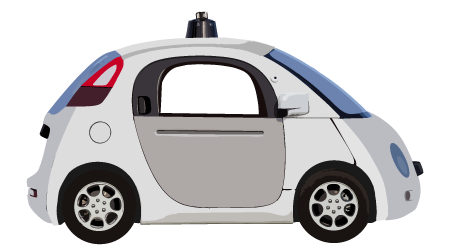
\includegraphics[width=\linewidth]{figs/car.png}\\
			\vspace{-0.2cm}
			\begin{center}
			\tiny{\href{http://www.national.co.uk/tech-powers-google-car/}{(Source)}}
			\end{center}
	\end{columns}

	Machine Learning
	\begin{itemize}
		\item Allows computers to do things without explicit programming
		\item Many techniques: Neural networks, decision trees, bayesian networks, ...
		\item Huge number of applications
		\item Hot topic nowdays (and job opportunities!)
	\end{itemize}
	
\end{frame}

\begin{frame}{AI applications}{Building HAL: Learning (II)}
	Another discipline: Expert systems
	\begin{itemize}
		\item It maintains a knowledge base, facts base and interence engine
		\item Expert systems can learn
	\end{itemize}
	Other approaches: Case Based Reasoning, Reinforcement Learning, probabilistic learning, Deep Learning, ...
	\begin{itemize}
		\item \href{https://www.youtube.com/watch?v=W_gxLKSsSIE}{(Video)}
	\end{itemize}
	Conclusion: YES
\end{frame}

\begin{frame}{AI applications}{Building HAL: Image recognition}
	Recognition vs. understanding (like speech)
	\begin{itemize}
		\item Applications: Face recognition, object recognition, object tracking, ... \href{https://www.youtube.com/watch?v=y5NWCjMbOZk}{(Video)}
		\item Techniques: Computer vision, Machine Learning, Deep Learning, ...
	\end{itemize}
	Again, it is a hard problem
	\begin{center}
		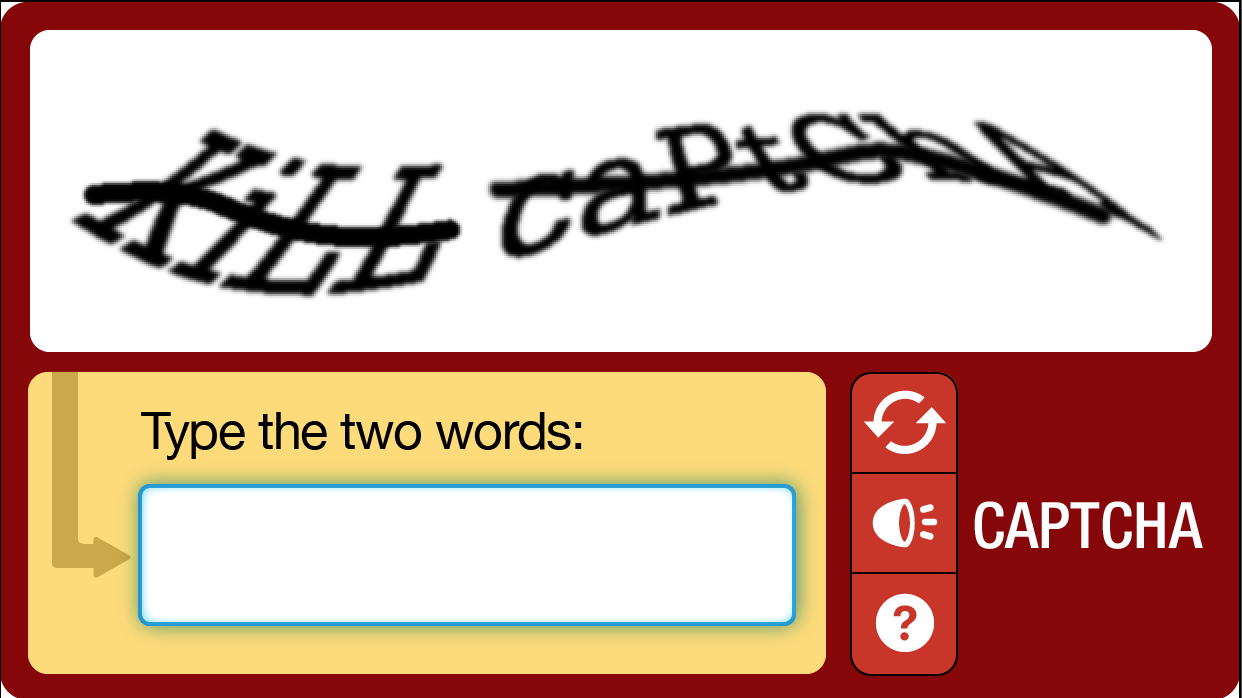
\includegraphics[width=0.25\linewidth]{figs/captcha.png}\\
		\tiny{\href{http://www.ohmygeek.net/2015/03/12/podec-troyano-captcha/}{(Source)}}
	\end{center}

	Conclusion: NO for general recognition, YES for restricted domains
\end{frame}

\begin{frame}{AI applications}{Building HAL: Plan and make decisions}
	Intelligence involves solving problems, making decisions and plans
	\begin{itemize}
		\item Plan: Sequence of actions to achieve a goal
		\item Techniques: Search
	\end{itemize}
	Example: You want to plan a trip to Caribe
	\begin{itemize}
		\item Decide on dates, flights, airport transport, hotel, fit timetables, ...
	\end{itemize}
	It is a hard problem
	\begin{itemize}
		\item World is not predecible (flights can be delayed)
		\item Huge number of details, common sense constrains decisions
	\end{itemize}
	Life-and-death decisions: \href{https://www.youtube.com/watch?v=ixIoDYVfKA0}{(Video)}

	Conclusion: NO for real-world planning, YES for restricted domains
\end{frame}

\subsection{Disciplines}
\begin{frame}{AI applications}{Disciplines and techniques}
	\vspace{-0.4cm}
	\begin{center}
		\textbf{AI disciplines techniques}
	\end{center}
	\begin{columns}
 	   \column{.50\textwidth}
	   		\begin{block}{Disciplines}
			\begin{itemize}
			\item Automatic reasoning
			\item Planning
			\item Agents
			\item Expert systems
			\item Computer vision
			\item Evolutionary Computation
			\item Natural Language Processing
			\item Machine Learning
			\item Knowledge representation
			\item ...
			\end{itemize}
			\end{block}
 	   \column{.50\textwidth}
	   		\begin{block}{Techniques}
			\begin{itemize}
			\item Neural networks
			\item Search algorithms
			\item Genetic Algorithms
			\item Case Based Reasoning
			\item Logic
			\item Fuzzy logic
			\item Web mining
			\item Ontologies
			\item ...
			\end{itemize}
			\end{block}
	\end{columns}
\end{frame}

\subsection{Application domains}

\begin{frame}{AI applications}{Application domains (I)}
	Genetic Algorithms
	\begin{itemize}
		\item Optimization of production chains
		\item Optimization of airline planes and crews
		\item Antenna design
	\end{itemize}
	Expert Systems
	\begin{itemize}
		\item Decision making in financial markets
		\item Fraud detection
		\item Medical diagnosis systems
	\end{itemize}
	Neural networks
	\begin{itemize}
		\item Face recognition
		\item Robot control
		\item OCR
	\end{itemize}
\end{frame}

\begin{frame}{AI applications}{Application domains (II)}
	\begin{itemize}
		\item Handwriting recognition (reading service postcodes USA) 
		\item Search engines on the Web and Semantic Web 
		\item Bio(logical) computing 
		\item Anti-spam email 
		\item Proof of theorems automatically 
			\begin{itemize}
			\item Using new methods of inference to prove new theorems
			\end{itemize}
	\end{itemize}
\end{frame}

\begin{frame}{AI applications}{Application domains (III)}
	\begin{itemize}
		\item Applied Problems 
		\item Pattern Recognition 
		\item Artificial Creativity 
		\item Machine Vision 
		\item Automatic diagnosis 
		\item Game Theory 
		\item Intelligent games and bots 
		\item Language Processing 
		\item Planning and scheduling 
		\item Nonlinear control 
		\item Learning …
	\end{itemize}	
\end{frame}

\begin{frame}{AI applications}{Application domains (IV)}
	AI in Robotics
	\begin{itemize}
		\item \href{http://www.youtube.com/watch?v=gDvoe091tk4}{(Video Athlete)}
		\item \href{https://www.youtube.com/watch?v=M8YjvHYbZ9w}{(Video Spot)}
		\item \href{https://www.youtube.com/watch?v=rVlhMGQgDkY}{(Video Atlas)}
		\item \href{https://www.youtube.com/watch?v=NhLi1LsNzno}{(Video ExoMars)}
		\item \href{http://www.jpl.nasa.gov/news/phoenix/multimedia.php}{(MSL Photos)}
%		\item \href{http://www.jpl.nasa.gov/news/phoenix/multimedia.php}{(Video MSL)}
%		\item \href{http://www.youtube.com/watch?v=JI6F1qrsQb0}{(Video MER)}
%		\item \href{http://www.youtube.com/watch?v=j72quVM7c9Y}{(Video Phoenix)}
%		\item \href{http://www.youtube.com/watch?v=d1coV7XqE1M}{(Video MSL)}
%		\item \href{http://www.youtube.com/watch?v=p-ho4IU30Ac}{(Video MSL landing)}
	\end{itemize}
\end{frame}


\IfStrEq{\modo}{MASTER-ESPACIO}{
	\section{AI in space}
	\subsection{Why is Mars interesting?}
	\begin{frame}{AI in space}{Why is Mars interesting? (I)}
		\footnotesize{
		\vspace{-0.2cm}
		\begin{columns}
 	   		\column{.01\textwidth}
 	   		\column{.7\textwidth}
				Mars is a lot like Earth
				\begin{itemize}
					\item About 1/2 size than Earth
					\item Martian day slightly under 25 hours
					\item Avg. temp -63º (-140ºC to 20ºC)
				\end{itemize}

 	  		\column{.2\textwidth}
	   			\vspace{0.5cm}
				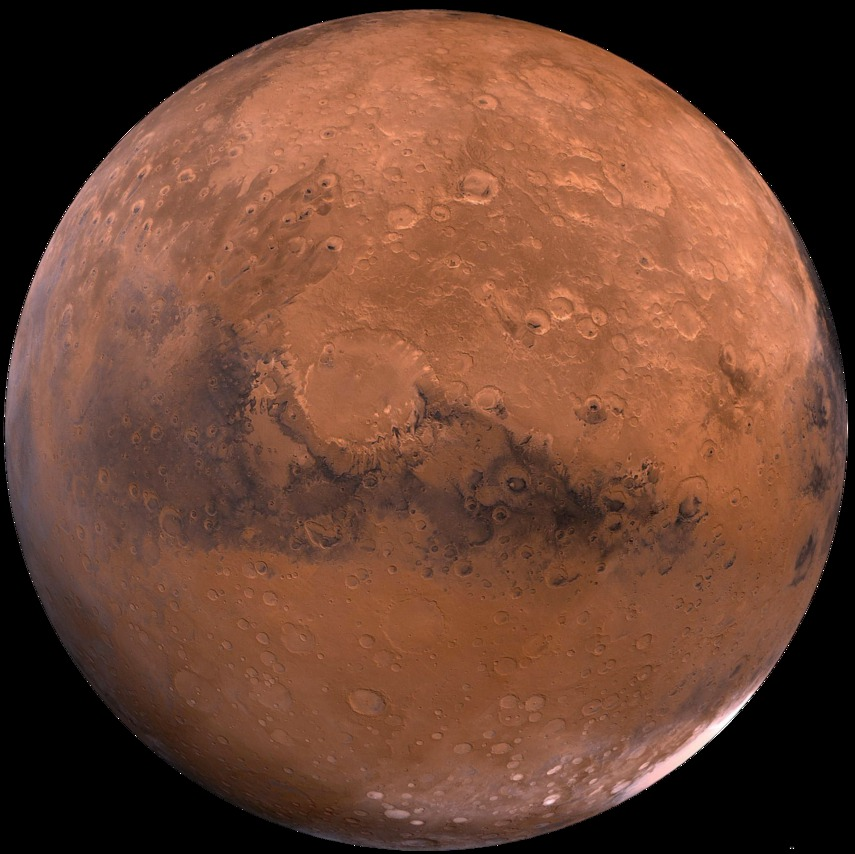
\includegraphics[width=\linewidth]{figs/marte-small.jpg}\\
				\vspace{-0.4cm}
				\begin{center}
				\tiny{\href{https://journalismfrommars.co.uk/}{(Source)}}
				\end{center}
 	   		\column{.05\textwidth}
		\end{columns}
		\vspace{-0.5cm}
		Distant past
		\begin{itemize}
			\item Evidence of oceans and warm temperatures
			\item It may have harbored life
		\end{itemize}
		Present
		\begin{itemize}
			\item Frozen water and a thin atmosphere of carbon dioxide remain
			\item It is possible that it harbors life today
			\item Earth is sending many robotic spacecraft to investigate
		\end{itemize}
		Future
		\begin{itemize}
			\item Mars has all of the materials needed to support human civilization
			\item Several nations interested in sending humans to Mars in the future
		\end{itemize}
		}
	\end{frame}

	\begin{frame}{AI in space}{Why is Mars interesting? (II)}
		\vspace{-0.2cm}
		\begin{center}
			Strong evidence of recent water activity\\
			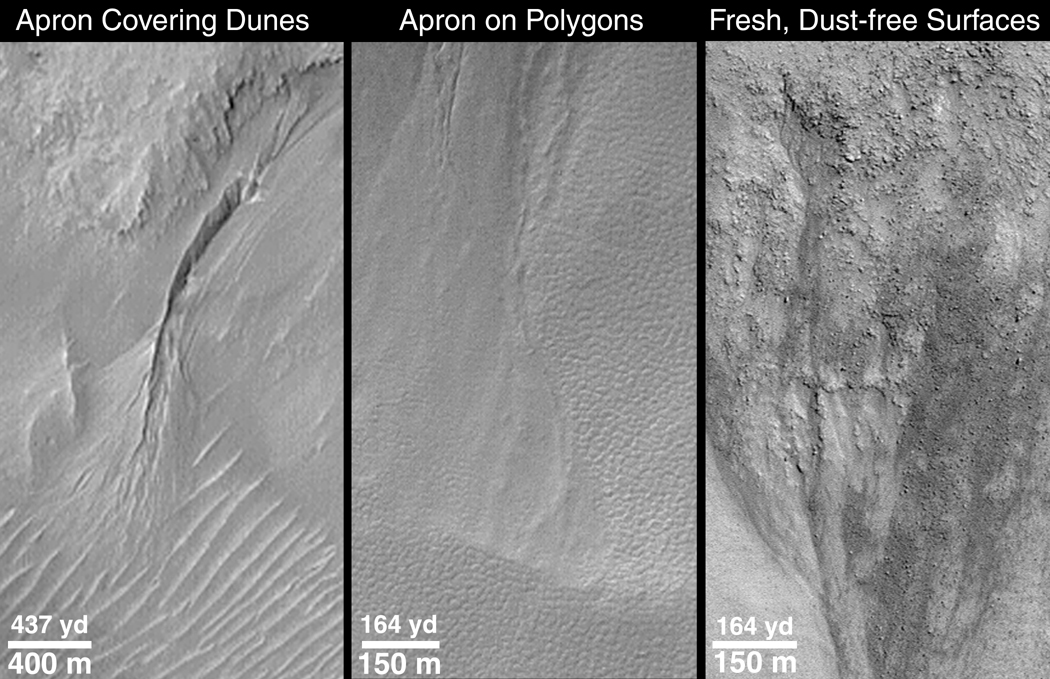
\includegraphics[width=0.8\linewidth]{figs/marswater.jpg}\\
			\tiny{\href{http://www.msss.com/mars_images/moc/june2000/age/index.html}{(Source)}}
		\end{center}
	\end{frame}

	\begin{frame}{AI in space}{Why is Mars interesting? (III)}
		\vspace{-0.2cm}
		\begin{center}
			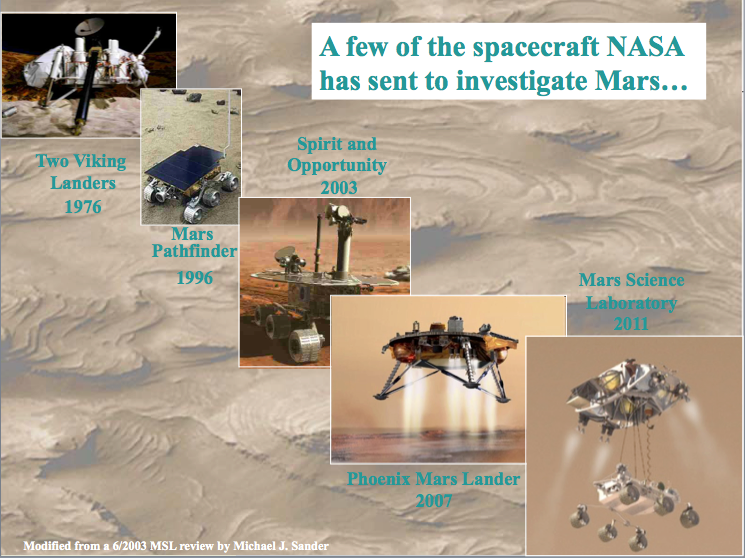
\includegraphics[width=0.8\linewidth]{figs/rovers.png}
		\end{center}
	\end{frame}

	\subsection{MER: Spirit and Opportunity}
	\begin{frame}{AI in space}{Spirit and Opportunity (I)}
		\begin{center}
			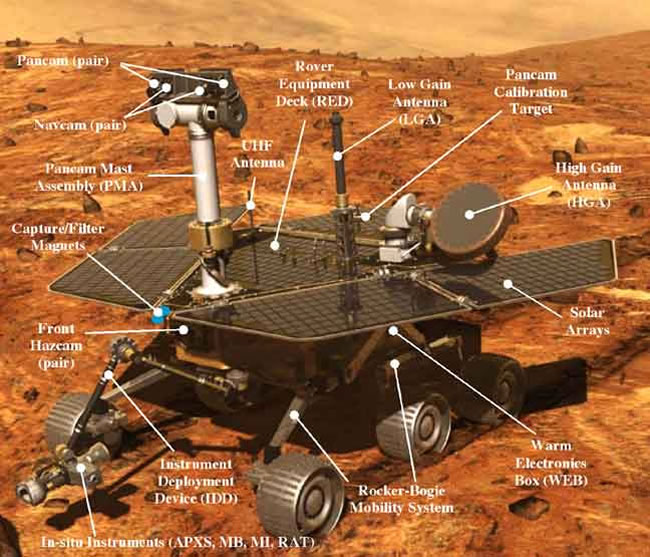
\includegraphics[width=0.6\linewidth]{figs/rover_detail_large.jpg}
		\end{center}
	\end{frame}

	\begin{frame}{AI in space}{Spirit and Opportunity (II)}
		\begin{center}
			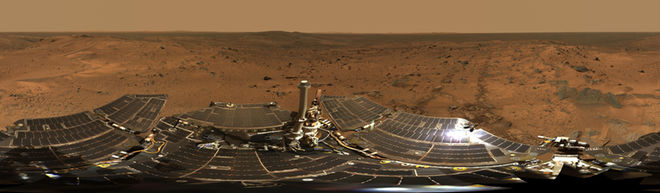
\includegraphics[width=0.9\linewidth]{figs/opportunity.jpg}
		\end{center}

		\vspace{-0.2cm}

		\begin{itemize}
			\item Some Mars rocks contain minerals that only form in water
			\item Some sediment layers were formed in standing water
			\item Mars was covered with standing water in the past
			\item Mars used to be much warmer and wetter
		\end{itemize}
	\end{frame}

	\begin{frame}{AI in space}{Spirit and Opportunity (III)}
		\vspace{-0.4cm}
		\begin{center}
		Clouds of water vapor on Mars\\\bigskip
			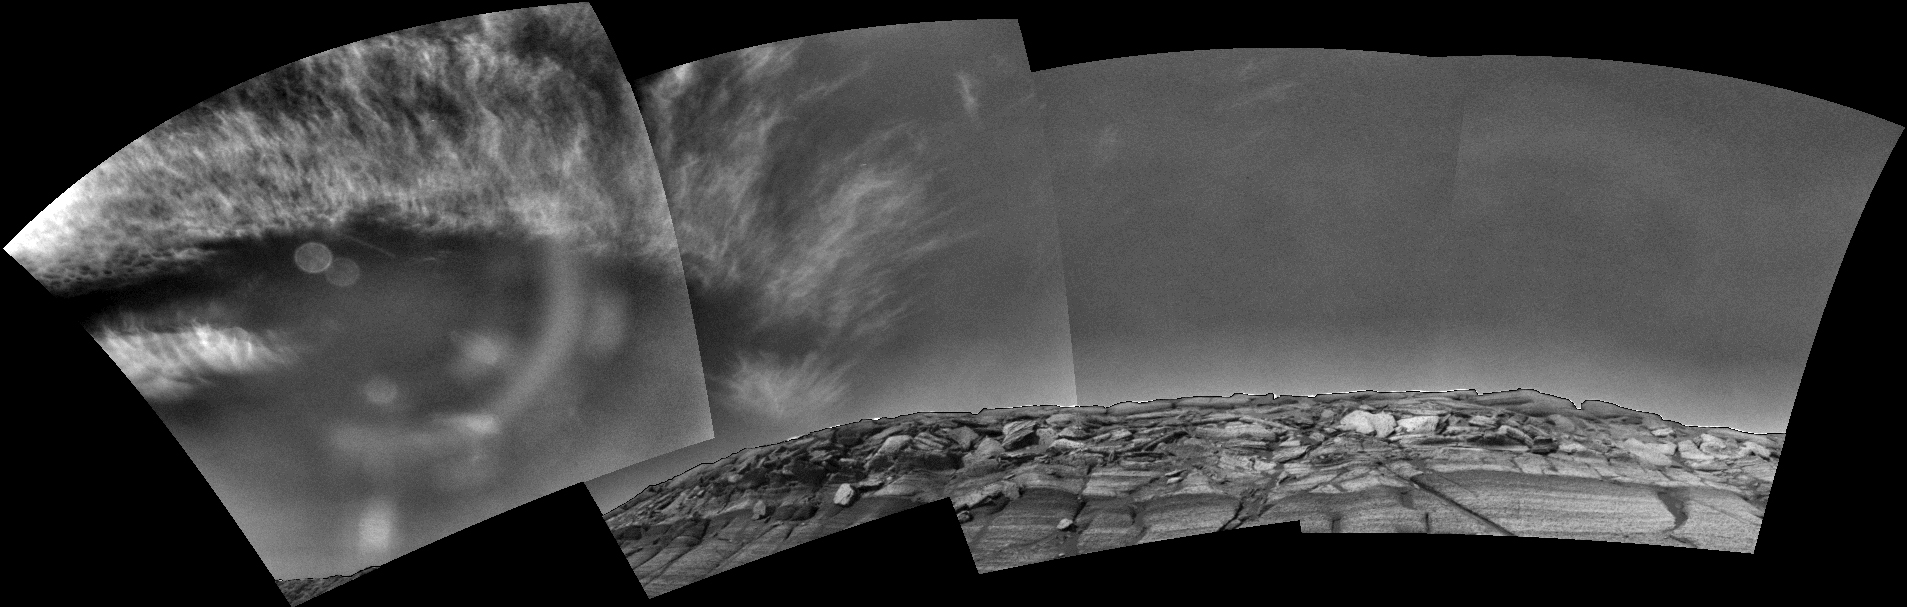
\includegraphics[width=0.9\linewidth]{figs/clouds.jpg}
		\end{center}

%		\href{https://www.youtube.com/watch?v=Auphov6TNy0}{(Spirit launch)} \href{https://www.youtube.com/watch?v=p1m9p2uomE8}{(Video MER by Steve Squyres)}
		\href{https://www.youtube.com/watch?v=LPKtuyB8E20}{(Video Sunset)} \href{https://www.youtube.com/watch?v=p1m9p2uomE8}{(Video MER by Steve Squyres)}
	\end{frame}

	\subsection{2007 Phoenix Mars Lander}
	\begin{frame}{AI in space}{2007 Phoenix Mars Lander (I)}
		\begin{columns}
 	   		\column{.01\textwidth}
 	   		\column{.6\textwidth}
				Launched August 2007
				\begin{itemize}
				\item Operated on Mars May-November 2008
				\end{itemize}

 	  		\column{.4\textwidth}
				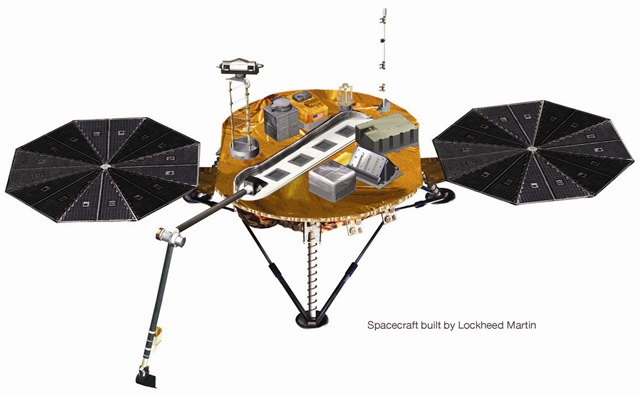
\includegraphics[width=\linewidth]{figs/phoenix.jpg}\\
		\end{columns}
		\vspace{-0.2cm}
		Goals
		\begin{itemize}
			\item Study the history of water in the Martian artic
			\item Search for evidence of a habitable zone and assess biological potential
		\end{itemize}
		How?
		\begin{itemize}
			\item Land in the Martian Arctic
			\item Dig through regolith to water ice
			\item Analyze ice samples in on-board
		\end{itemize}
	\end{frame}

	\begin{frame}{AI in space}{2007 Phoenix Mars Lander (II)}
		\vspace{-0.5cm}
		\begin{center}
			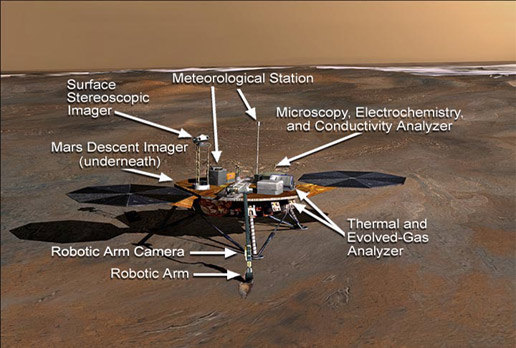
\includegraphics[width=0.8\linewidth]{figs/phoenixinstruments.jpg}
		\end{center}
	\end{frame}

	\begin{frame}{AI in space}{2007 Phoenix Mars Lander (III)}
		\vspace{-0.5cm}
		\begin{center}
			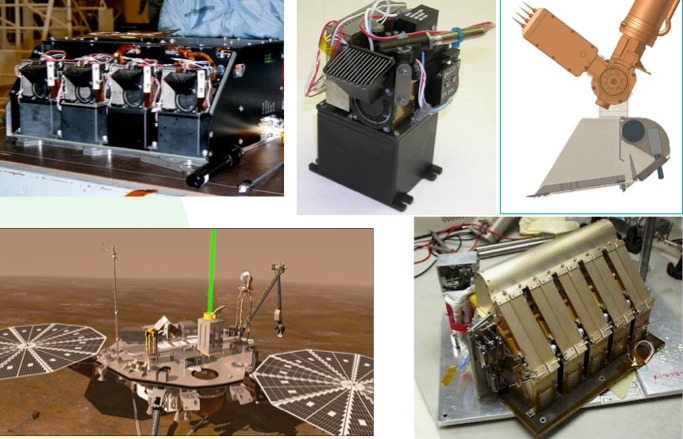
\includegraphics[width=0.8\linewidth]{figs/instrumentsPhoenix.jpg}
		\end{center}
	\end{frame}

	\begin{frame}{AI in space}{2007 Phoenix Mars Lander (IV)}
		\vspace{-0.5cm}
		\begin{center}
			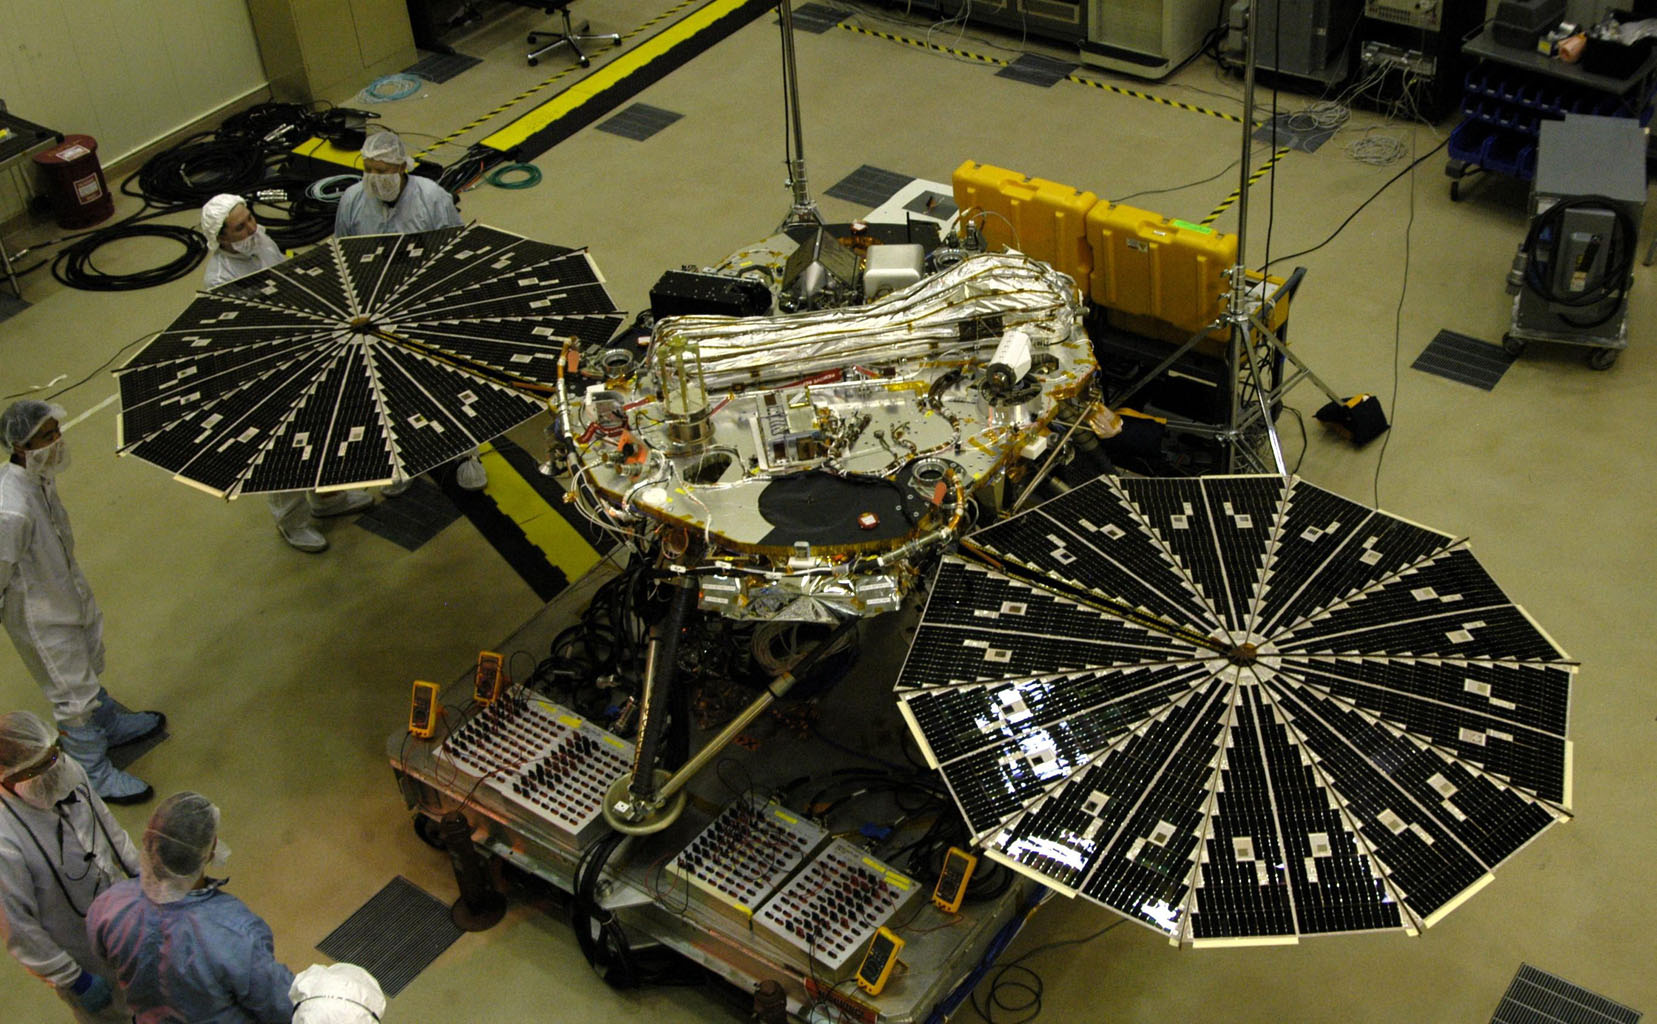
\includegraphics[width=0.8\linewidth]{figs/testing.jpg}
		\end{center}
	\end{frame}

	\begin{frame}{AI in space}{2007 Phoenix Mars Lander (V)}
		\vspace{-2cm}
		\begin{center}
			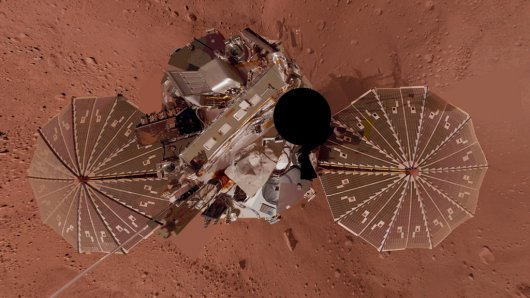
\includegraphics[width=0.8\linewidth]{figs/lander.jpg}
		\end{center}
		\vspace{-6.2cm}
		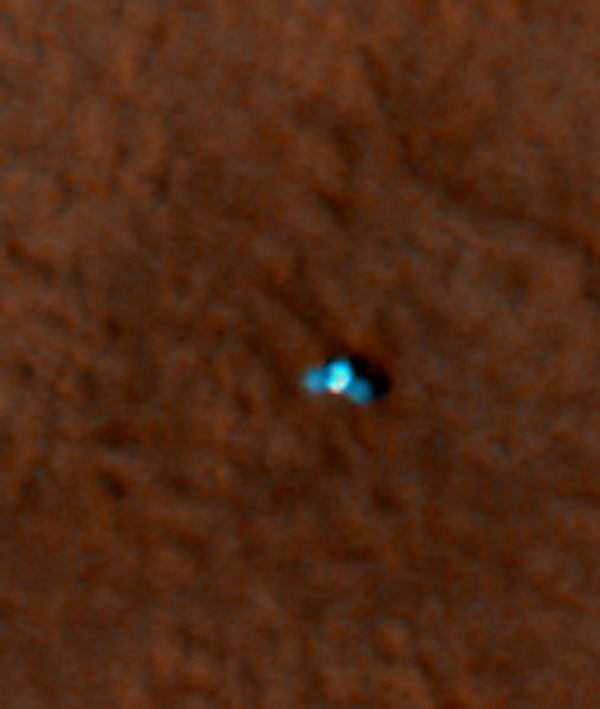
\includegraphics[width=0.2\linewidth]{figs/mro.jpg}
	\end{frame}

	\begin{frame}{AI in space}{2007 Phoenix Mars Lander (VI)}
		\vspace{-0.2cm}

		\begin{center}
			Phoenix achievements\\
			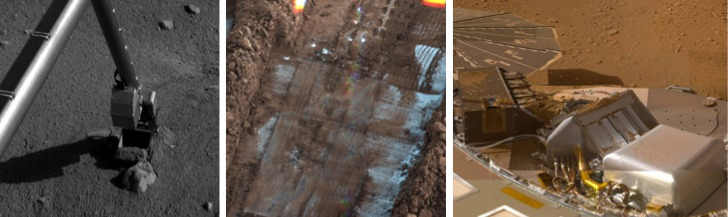
\includegraphics[width=0.7\linewidth]{figs/logrosPhoenix.jpg}
		\end{center}

		\vspace{-0.5cm}

		\begin{itemize}
		\item Observed and sampled water ice in the Martian arctic
		\item Studied the water cycle 
			\begin{itemize}
		 	\item Sublimation of ice, precipitation of ice crystals (snow)
		  	\item Evidence that a liquid water film can form in the soil
			\end{itemize}
		\item Studied chemical makeup of the soil 
		  	\begin{itemize}
		   	\item Salts that typically form in presence of liquid water
		    \item Perchlorates that could be an energy source for life	
			\end{itemize}
		\end{itemize}
	\end{frame}

	\begin{frame}{AI in space}{2007 Phoenix Mars Lander (VII)}
		\begin{center}
			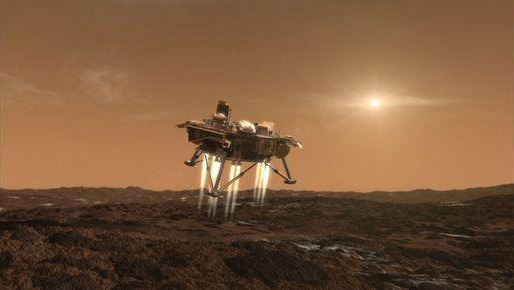
\includegraphics[width=0.8\linewidth]{figs/phoenix_landing.jpg}\\
			\href{https://www.youtube.com/watch?v=j72quVM7c9Y}{(Video)}
		\end{center}
	\end{frame}

	\subsection{MSL}
	\begin{frame}{AI in space}{MSL (I)}
		\begin{center}
			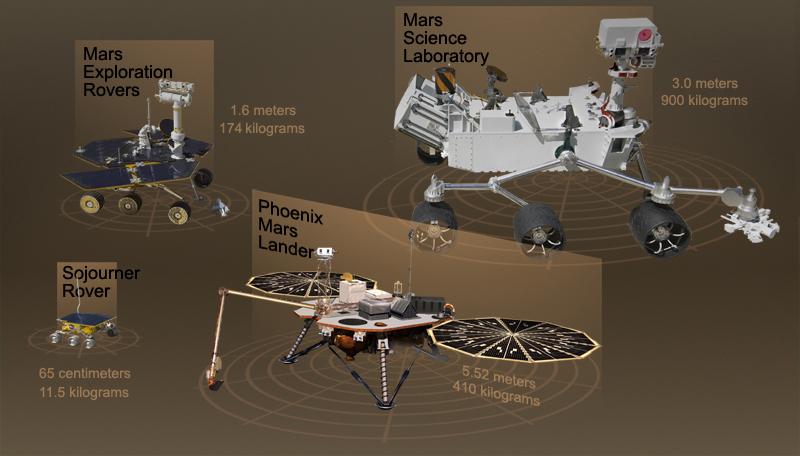
\includegraphics[width=0.8\linewidth]{figs/comparison.jpg}
		\end{center}
	\end{frame}

	\begin{frame}{AI in space}{MSL (II)}
		\begin{center}
			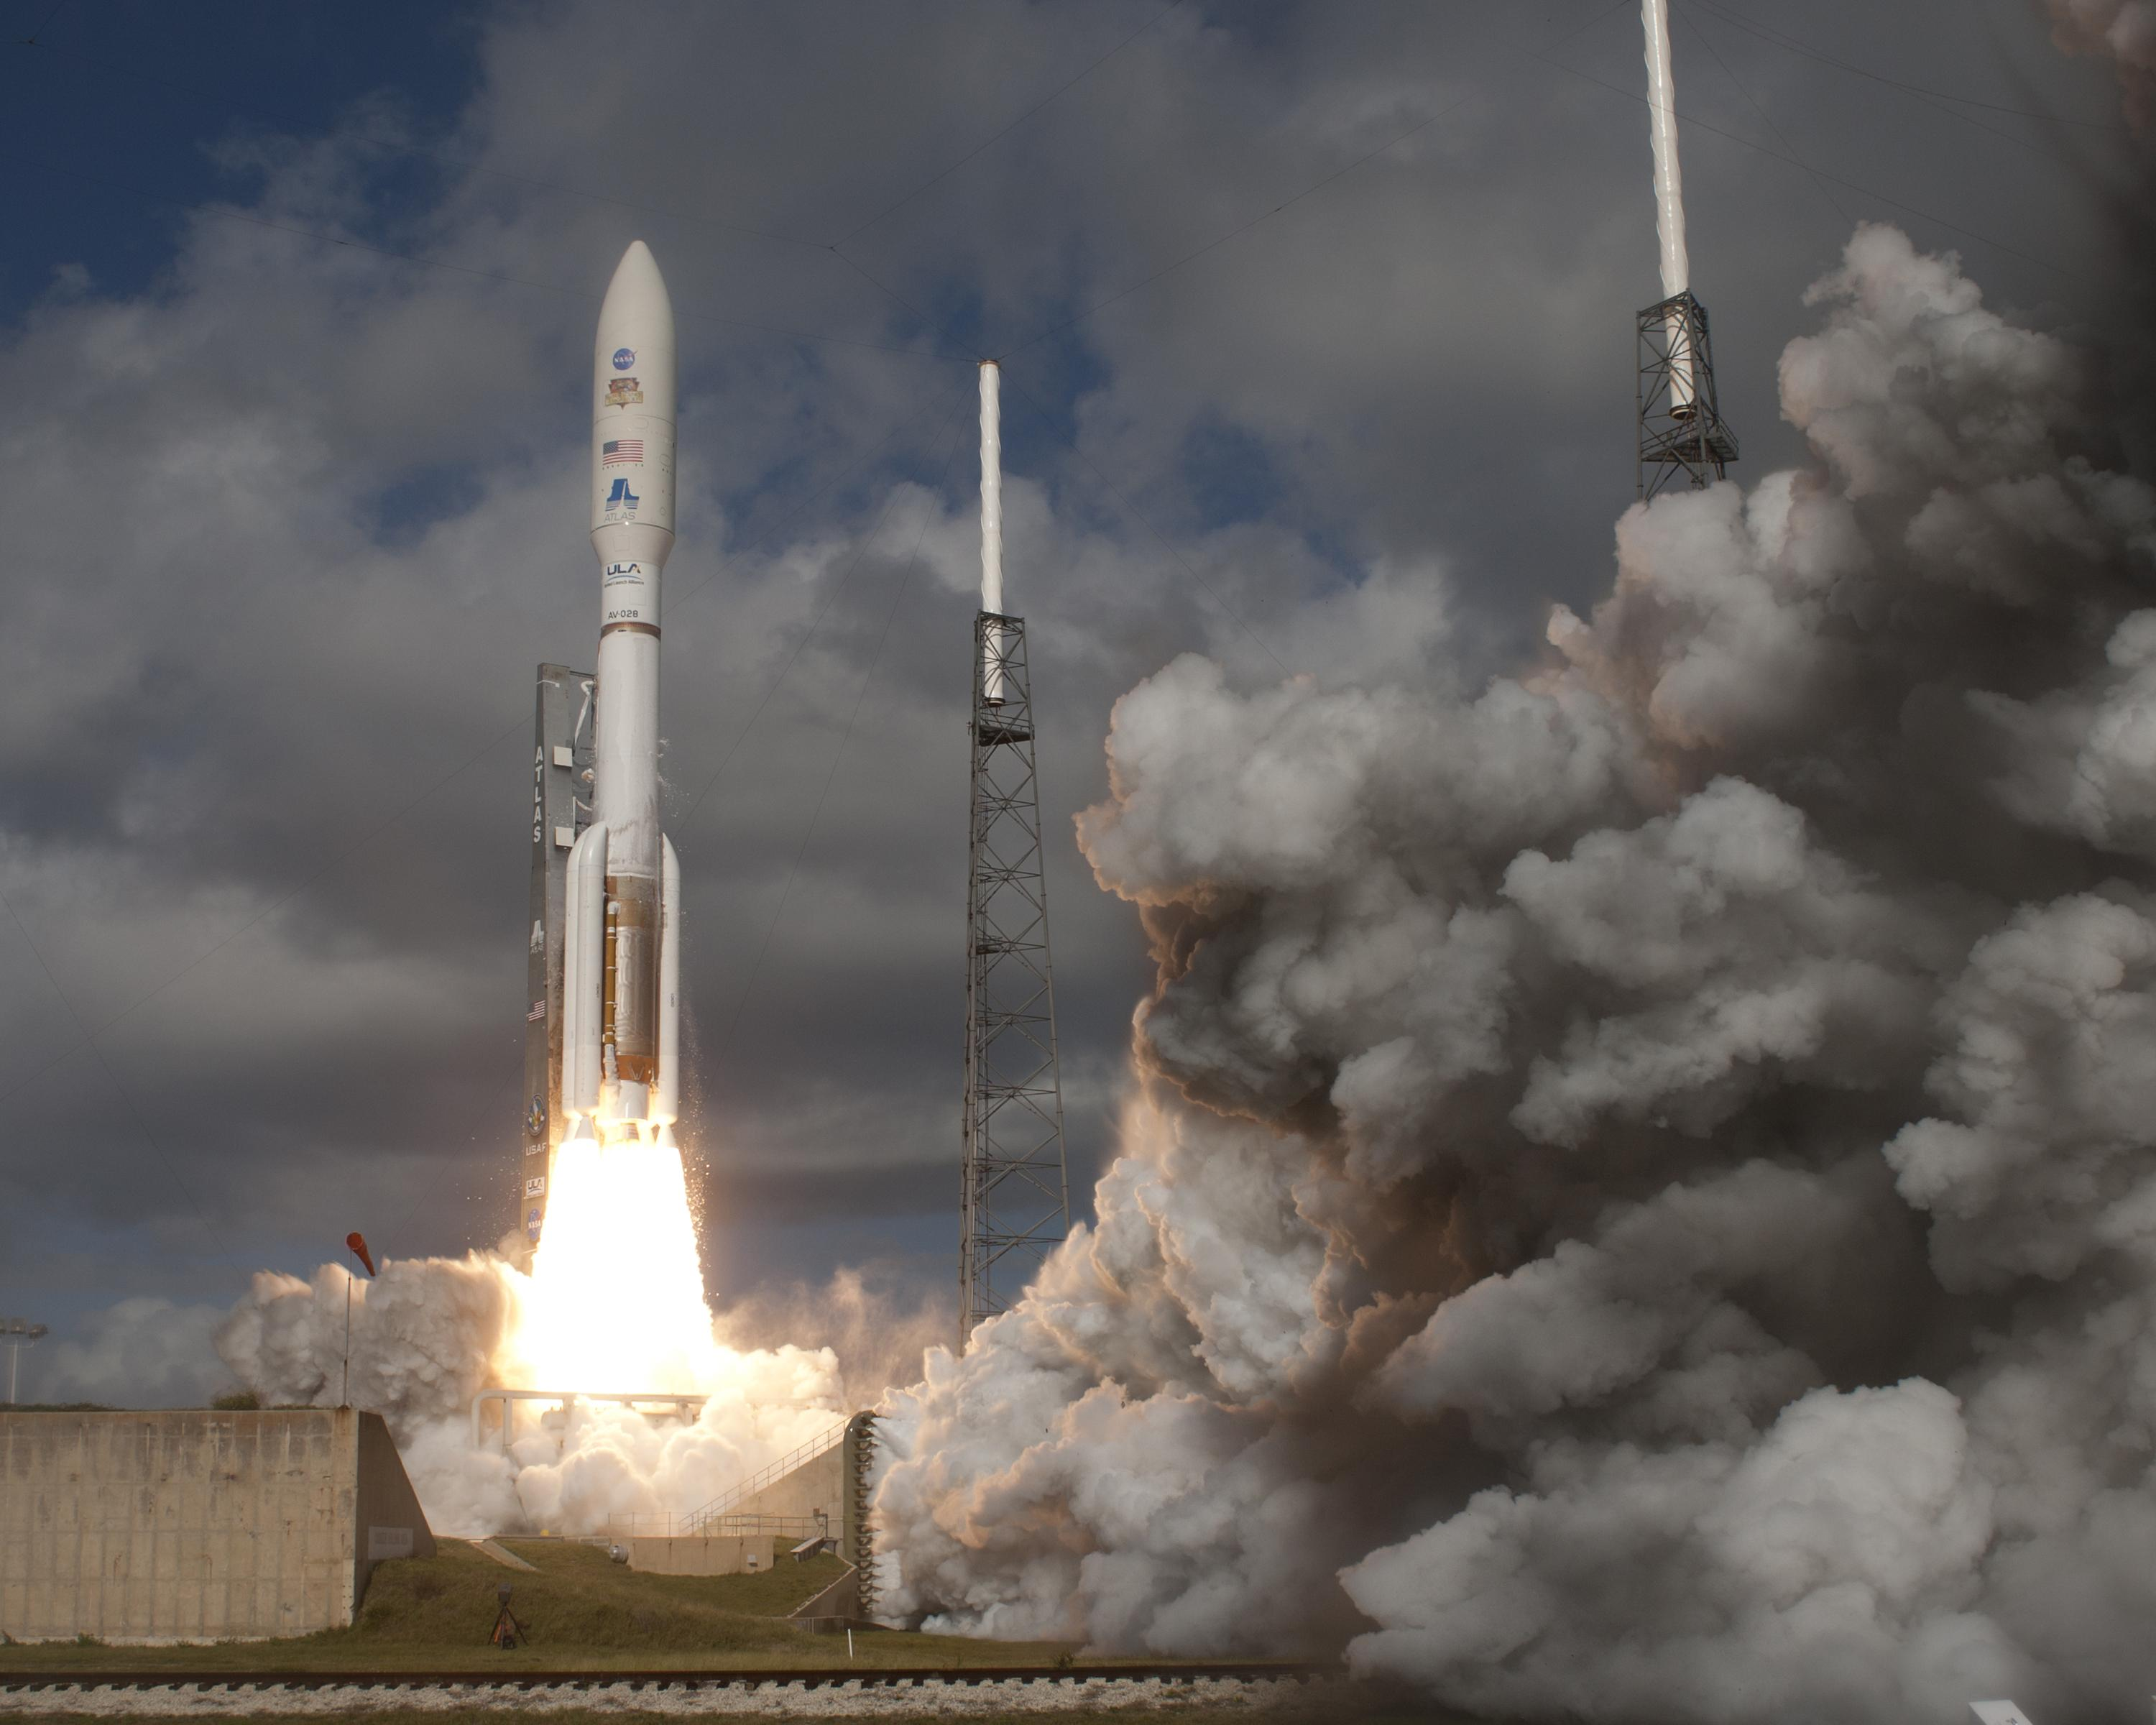
\includegraphics[width=0.4\linewidth]{figs/msllaunch.jpg}
		\end{center}
		\begin{itemize}
			\item Launch: Nov. 26, 2011
			\begin{itemize}
				\item Inside Atlas V rocket
		 		\item Cape Canaveral Air Force Station in Florida
			\end{itemize}
		 	\item The spacecraft arrived at Mars in August 2012
		\end{itemize}
	\end{frame}

	\begin{frame}{AI in space}{MSL (III)}
		\vspace{-0.2cm}
		\begin{center}
			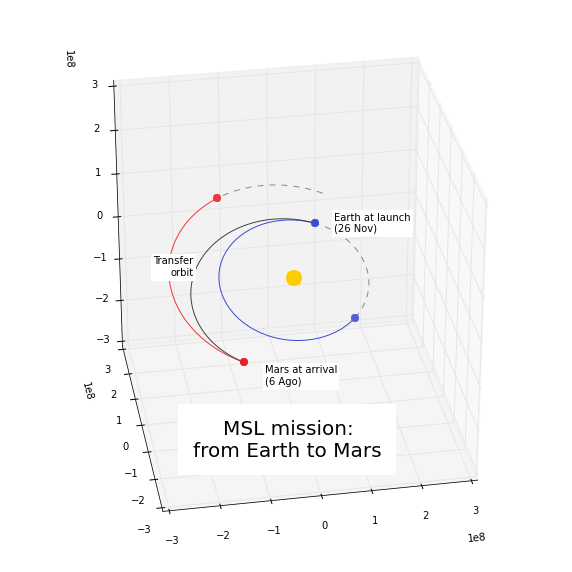
\includegraphics[width=0.6\linewidth]{figs/mslorbit.png}\\
			\tiny{\href{http://poliastro.readthedocs.org/en/latest/user_guide.html}{(Source)}}
		\end{center}
	\end{frame}

	\begin{frame}{AI in space}{MSL (IV)}
		\begin{columns}
 	  		\column{.4\textwidth}
				\begin{center}
					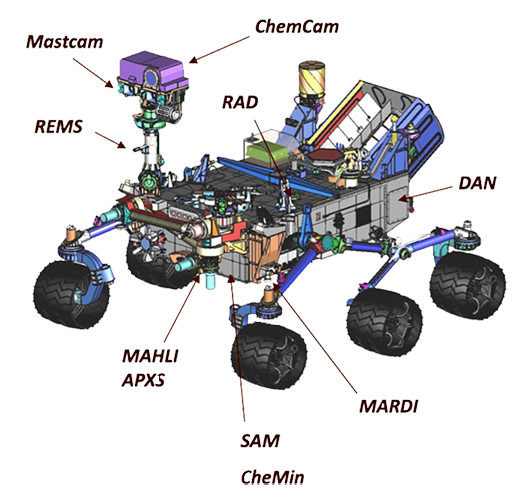
\includegraphics[width=\linewidth]{figs/msl.png}\\
					\tiny{\href{http://www.msl-chemcam.com/}{(Source)}}
				\end{center}
			\column{.6\textwidth}
				\footnotesize{
				\begin{itemize}
					\item Mast Camera (Mastcam) 
					\item Chemistry \& Camera (ChemCam) 
					\item Alpha Particle X-ray Spectrometer (APXS) 
					\item Mars Hand Lens Imager (MAHLI) 
			 		\item Chemistry \& Mineralogy (CheMin) 
			 		\item Sample Analysis at Mars (SAM) 
			 		\item Radiation Assessment Detector (RAD) 
			 		\item Rover Environmental Monitoring Station (REMS) 
			 		\item Dynamic Albedo of Neutrons (DAN)
			  		\item Mars Descent Imager (MARDI5)
				\end{itemize}
				}
		\end{columns}
	\end{frame}

	\begin{frame}{AI in space}{MSL (V)}
		MSL goals (Primary mission 687 days)
		\begin{itemize}
			\item Assess potential habitat for life, past or present
			\item Assess biological potential...
			\item Characterize the geology of the landing region ...
			\item Investigate processes relevant to past habitability...
			\item Characterize surface radiation...
		\end{itemize}
		Instruments include
		\begin{itemize}
			\item Chemcam
			\item Variety of spectrometers 
			\item Subsurface water detection
		\end{itemize}
		\href{https://www.youtube.com/watch?v=p-ho4IU30Ac}{(Video MSL)}
		\href{https://www.youtube.com/watch?v=Ki_Af_o9Q9s}{(Video Landing Process MSL)}

		\vspace{-3cm}
		\begin{flushright}
			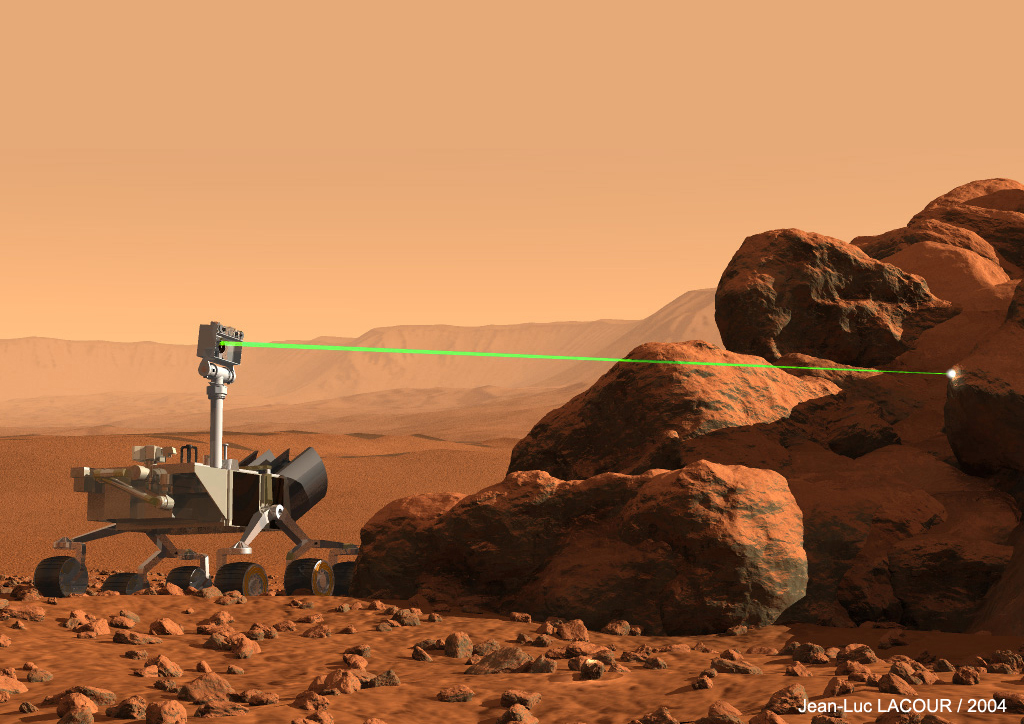
\includegraphics[width=0.4\linewidth]{figs/chemcam.jpg}
		\end{flushright}
	\end{frame}
}{}

\begin{frame}[plain]{}
	\begin{columns}
 	   \column{.50\textwidth}
			\begin{block}{Collorary}
			AI addresses the automatic problems resolution
			\end{block}
	\end{columns}
\end{frame}

%\begin{frame}{Acknowlegements}
%	\begin{itemize}
%		\item Professor Padhraic Smyth, University of California, Irvine. 
%	\end{itemize}
%\end{frame}

\end{document}
